\documentclass[12pt,]{article}
\usepackage{lmodern}
\usepackage{amssymb,amsmath}
\usepackage{ifxetex,ifluatex}
\usepackage{fixltx2e} % provides \textsubscript
\ifnum 0\ifxetex 1\fi\ifluatex 1\fi=0 % if pdftex
  \usepackage[T1]{fontenc}
  \usepackage[utf8]{inputenc}
\else % if luatex or xelatex
  \ifxetex
    \usepackage{mathspec}
  \else
    \usepackage{fontspec}
  \fi
  \defaultfontfeatures{Ligatures=TeX,Scale=MatchLowercase}
    \setmainfont[]{TeX Gyre Pagella}
\fi
% use upquote if available, for straight quotes in verbatim environments
\IfFileExists{upquote.sty}{\usepackage{upquote}}{}
% use microtype if available
\IfFileExists{microtype.sty}{%
\usepackage{microtype}
\UseMicrotypeSet[protrusion]{basicmath} % disable protrusion for tt fonts
}{}
\usepackage[left=2.5cm,right=2.5cm,top=2.5cm,bottom=2.5cm]{geometry}
\usepackage{hyperref}
\hypersetup{unicode=true,
            pdftitle={Supplementary materials for: Modelling palaeoecological time series using generalized additive models},
            pdfauthor={Gavin L. Simpson},
            pdfkeywords={time series; generalized additive model; simultaneous interval; spline;
environmental change},
            pdfborder={0 0 0},
            breaklinks=true}
\urlstyle{same}  % don't use monospace font for urls
\usepackage{color}
\usepackage{fancyvrb}
\newcommand{\VerbBar}{|}
\newcommand{\VERB}{\Verb[commandchars=\\\{\}]}
\DefineVerbatimEnvironment{Highlighting}{Verbatim}{commandchars=\\\{\}}
% Add ',fontsize=\small' for more characters per line
\usepackage{framed}
\definecolor{shadecolor}{RGB}{248,248,248}
\newenvironment{Shaded}{\begin{snugshade}}{\end{snugshade}}
\newcommand{\KeywordTok}[1]{\textcolor[rgb]{0.13,0.29,0.53}{\textbf{{#1}}}}
\newcommand{\DataTypeTok}[1]{\textcolor[rgb]{0.13,0.29,0.53}{{#1}}}
\newcommand{\DecValTok}[1]{\textcolor[rgb]{0.00,0.00,0.81}{{#1}}}
\newcommand{\BaseNTok}[1]{\textcolor[rgb]{0.00,0.00,0.81}{{#1}}}
\newcommand{\FloatTok}[1]{\textcolor[rgb]{0.00,0.00,0.81}{{#1}}}
\newcommand{\ConstantTok}[1]{\textcolor[rgb]{0.00,0.00,0.00}{{#1}}}
\newcommand{\CharTok}[1]{\textcolor[rgb]{0.31,0.60,0.02}{{#1}}}
\newcommand{\SpecialCharTok}[1]{\textcolor[rgb]{0.00,0.00,0.00}{{#1}}}
\newcommand{\StringTok}[1]{\textcolor[rgb]{0.31,0.60,0.02}{{#1}}}
\newcommand{\VerbatimStringTok}[1]{\textcolor[rgb]{0.31,0.60,0.02}{{#1}}}
\newcommand{\SpecialStringTok}[1]{\textcolor[rgb]{0.31,0.60,0.02}{{#1}}}
\newcommand{\ImportTok}[1]{{#1}}
\newcommand{\CommentTok}[1]{\textcolor[rgb]{0.56,0.35,0.01}{\textit{{#1}}}}
\newcommand{\DocumentationTok}[1]{\textcolor[rgb]{0.56,0.35,0.01}{\textbf{\textit{{#1}}}}}
\newcommand{\AnnotationTok}[1]{\textcolor[rgb]{0.56,0.35,0.01}{\textbf{\textit{{#1}}}}}
\newcommand{\CommentVarTok}[1]{\textcolor[rgb]{0.56,0.35,0.01}{\textbf{\textit{{#1}}}}}
\newcommand{\OtherTok}[1]{\textcolor[rgb]{0.56,0.35,0.01}{{#1}}}
\newcommand{\FunctionTok}[1]{\textcolor[rgb]{0.00,0.00,0.00}{{#1}}}
\newcommand{\VariableTok}[1]{\textcolor[rgb]{0.00,0.00,0.00}{{#1}}}
\newcommand{\ControlFlowTok}[1]{\textcolor[rgb]{0.13,0.29,0.53}{\textbf{{#1}}}}
\newcommand{\OperatorTok}[1]{\textcolor[rgb]{0.81,0.36,0.00}{\textbf{{#1}}}}
\newcommand{\BuiltInTok}[1]{{#1}}
\newcommand{\ExtensionTok}[1]{{#1}}
\newcommand{\PreprocessorTok}[1]{\textcolor[rgb]{0.56,0.35,0.01}{\textit{{#1}}}}
\newcommand{\AttributeTok}[1]{\textcolor[rgb]{0.77,0.63,0.00}{{#1}}}
\newcommand{\RegionMarkerTok}[1]{{#1}}
\newcommand{\InformationTok}[1]{\textcolor[rgb]{0.56,0.35,0.01}{\textbf{\textit{{#1}}}}}
\newcommand{\WarningTok}[1]{\textcolor[rgb]{0.56,0.35,0.01}{\textbf{\textit{{#1}}}}}
\newcommand{\AlertTok}[1]{\textcolor[rgb]{0.94,0.16,0.16}{{#1}}}
\newcommand{\ErrorTok}[1]{\textcolor[rgb]{0.64,0.00,0.00}{\textbf{{#1}}}}
\newcommand{\NormalTok}[1]{{#1}}
\usepackage{graphicx,grffile}
\makeatletter
\def\maxwidth{\ifdim\Gin@nat@width>\linewidth\linewidth\else\Gin@nat@width\fi}
\def\maxheight{\ifdim\Gin@nat@height>\textheight\textheight\else\Gin@nat@height\fi}
\makeatother
% Scale images if necessary, so that they will not overflow the page
% margins by default, and it is still possible to overwrite the defaults
% using explicit options in \includegraphics[width, height, ...]{}
\setkeys{Gin}{width=\maxwidth,height=\maxheight,keepaspectratio}
\IfFileExists{parskip.sty}{%
\usepackage{parskip}
}{% else
\setlength{\parindent}{0pt}
\setlength{\parskip}{6pt plus 2pt minus 1pt}
}
\setlength{\emergencystretch}{3em}  % prevent overfull lines
\providecommand{\tightlist}{%
  \setlength{\itemsep}{0pt}\setlength{\parskip}{0pt}}
\setcounter{secnumdepth}{5}
% Redefines (sub)paragraphs to behave more like sections
\ifx\paragraph\undefined\else
\let\oldparagraph\paragraph
\renewcommand{\paragraph}[1]{\oldparagraph{#1}\mbox{}}
\fi
\ifx\subparagraph\undefined\else
\let\oldsubparagraph\subparagraph
\renewcommand{\subparagraph}[1]{\oldsubparagraph{#1}\mbox{}}
\fi

%%% Use protect on footnotes to avoid problems with footnotes in titles
\let\rmarkdownfootnote\footnote%
\def\footnote{\protect\rmarkdownfootnote}

%%% Change title format to be more compact
\usepackage{titling}

% Create subtitle command for use in maketitle
\newcommand{\subtitle}[1]{
  \posttitle{
    \begin{center}\large#1\end{center}
    }
}

\setlength{\droptitle}{-2em}
  \title{Supplementary materials for: Modelling palaeoecological time series
using generalized additive models}
  \pretitle{\vspace{\droptitle}\centering\huge}
  \posttitle{\par}
  \author{Gavin L. Simpson}
  \preauthor{\centering\large\emph}
  \postauthor{\par}
  \predate{\centering\large\emph}
  \postdate{\par}
  \date{May 13, 2018}

%\setromanfont{Constantia}
%\setromanfont{texgyrepagella.otf}
%\setmainfont{XITS}
%\setmathfont{XITS Math}
\setmathfont{TeX Gyre Pagella Math}
\setmathfont[range={\mathcal,\mathbfcal},StylisticSet=1]{XITS Math}

%\renewcommand\familydefault{\rmdefault} %comment to see the difference
%\DeclareMathAlphabet      {\mathup}{OT1}{\familydefault}{m}{n}

\newcommand{\uk}{\ensuremath{\mathit{U}^{\mathit{K}}_{\mathup{37}}}}

\newcommand{\loess}{\textsc{Loess}}

\usepackage{lineno}
\linenumbers

\begin{document}
\maketitle

\section{Introduction}\label{introduction}

This document is an annotated version of the R code used to fit the GAMs
and related analyses to the Small Water and Braya-Sø example data sets.

The following packages are required: \emph{mgcv}, \emph{scam},
\emph{ggplot2}, \emph{cowplot}, and \emph{tidyr}. Also, the
\emph{schoenberg} package is required; it is not on CRAN but can be
installed from Github.

\begin{Shaded}
\begin{Highlighting}[]
\KeywordTok{library}\NormalTok{(}\StringTok{"mgcv"}\NormalTok{)}
\end{Highlighting}
\end{Shaded}

\begin{verbatim}
#> Loading required package: nlme
\end{verbatim}

\begin{verbatim}
#> This is mgcv 1.8-23. For overview type 'help("mgcv-package")'.
\end{verbatim}

\begin{Shaded}
\begin{Highlighting}[]
\KeywordTok{library}\NormalTok{(}\StringTok{"scam"}\NormalTok{)}
\end{Highlighting}
\end{Shaded}

\begin{verbatim}
#> This is scam 1.2-2.
\end{verbatim}

\begin{Shaded}
\begin{Highlighting}[]
\KeywordTok{library}\NormalTok{(}\StringTok{"ggplot2"}\NormalTok{)}
\KeywordTok{library}\NormalTok{(}\StringTok{"cowplot"}\NormalTok{)}
\end{Highlighting}
\end{Shaded}

\begin{verbatim}
#> 
#> Attaching package: 'cowplot'
\end{verbatim}

\begin{verbatim}
#> The following object is masked from 'package:ggplot2':
#> 
#>     ggsave
\end{verbatim}

\begin{Shaded}
\begin{Highlighting}[]
\NormalTok{## schoenberg is not on CRAN, install from github:}
\NormalTok{## install.packages("devtools")}
\NormalTok{## devtools::install_github("gavinsimpson/schoenberg")}
\KeywordTok{library}\NormalTok{(}\StringTok{"schoenberg"}\NormalTok{)}
\KeywordTok{library}\NormalTok{(}\StringTok{"tidyr"}\NormalTok{)}

\NormalTok{## Default ggplot theme}
\KeywordTok{theme_set}\NormalTok{(}\KeywordTok{theme_bw}\NormalTok{())}
\end{Highlighting}
\end{Shaded}

The example data sets are also stored on github;
\url{https://github.com/gavinsimpson/frontiers-palaeo-additive-modelling}.
Once downloaded the data are read in and processed a little

\begin{Shaded}
\begin{Highlighting}[]
\NormalTok{## source Small Water data}
\NormalTok{small <-}\StringTok{ }\KeywordTok{readRDS}\NormalTok{(}\StringTok{"./data/small-water/small-water-isotope-data.rds"}\NormalTok{)}
\KeywordTok{head}\NormalTok{(small)}
\end{Highlighting}
\end{Shaded}

\begin{verbatim}
#>   Depth   d13C  TotalC d15N TotalN DryWeight     Year
#> 1   0.2 -27.57  806.49 3.05  64.21       8.2 2007.254
#> 2   0.4 -27.67  949.33 3.01  73.26       7.6 2006.510
#> 3   0.8 -27.63 1305.52 2.93  93.25      11.6 2004.941
#> 4   1.2 -27.62 1136.04 2.33  86.09       9.6 2003.269
#> 5   1.6 -27.48 1028.27 2.09  93.80      10.9 2001.496
#> 6   2.0 -27.39  809.91 2.66  79.98       9.9 1999.626
\end{verbatim}

\begin{Shaded}
\begin{Highlighting}[]
\NormalTok{## load braya so data set}
\NormalTok{braya <-}\StringTok{ }\KeywordTok{read.table}\NormalTok{(}\StringTok{"./data/braya-so/DAndrea.2011.Lake Braya So.txt"}\NormalTok{,}
                    \DataTypeTok{skip =} \DecValTok{84}\NormalTok{)}
\KeywordTok{names}\NormalTok{(braya) <-}\StringTok{ }\KeywordTok{c}\NormalTok{(}\StringTok{"Depth"}\NormalTok{, }\StringTok{"DepthUpper"}\NormalTok{, }\StringTok{"DepthLower"}\NormalTok{, }\StringTok{"Year"}\NormalTok{, }\StringTok{"YearYoung"}\NormalTok{,}
                  \StringTok{"YearOld"}\NormalTok{, }\StringTok{"UK37"}\NormalTok{)}
\NormalTok{braya <-}\StringTok{ }\KeywordTok{transform}\NormalTok{(braya, }\DataTypeTok{sampleInterval =} \NormalTok{YearYoung -}\StringTok{ }\NormalTok{YearOld)}
\KeywordTok{head}\NormalTok{(braya)}
\end{Highlighting}
\end{Shaded}

\begin{verbatim}
#>   Depth DepthUpper DepthLower     Year YearYoung YearOld   UK37
#> 1  0.25        0.0        0.5 1999.125   2006.00 1992.25 -0.640
#> 2  0.75        0.5        1.0 1985.375   1992.25 1978.50 -0.637
#> 3  1.25        1.0        1.5 1971.525   1978.50 1964.55 -0.614
#> 4  1.75        1.5        2.0 1957.575   1964.55 1950.60 -0.627
#> 5  2.25        2.0        2.5 1943.150   1950.60 1935.70 -0.633
#> 6  2.75        2.5        3.0 1928.250   1935.70 1920.80 -0.616
#>   sampleInterval
#> 1          13.75
#> 2          13.75
#> 3          13.95
#> 4          13.95
#> 5          14.90
#> 6          14.90
\end{verbatim}

\begin{Shaded}
\begin{Highlighting}[]
\NormalTok{## plot labels}
\NormalTok{d15n_label <-}\StringTok{ }\KeywordTok{expression}\NormalTok{(delta^\{}\DecValTok{15}\NormalTok{\}*N)}
\NormalTok{braya_ylabel <-}\StringTok{ }\KeywordTok{expression}\NormalTok{(}\KeywordTok{italic}\NormalTok{(U)[}\DecValTok{37}\NormalTok{]^\{}\KeywordTok{italic}\NormalTok{(k)\})}
\end{Highlighting}
\end{Shaded}

Plots of the two data sets are prepared using \emph{ggplot2}

\begin{Shaded}
\begin{Highlighting}[]
\NormalTok{## plot Small Water data}
\NormalTok{small_plt <-}\StringTok{ }\KeywordTok{ggplot}\NormalTok{(small, }\KeywordTok{aes}\NormalTok{(}\DataTypeTok{x =} \NormalTok{Year, }\DataTypeTok{y =} \NormalTok{d15N)) +}
\StringTok{    }\KeywordTok{geom_point}\NormalTok{() +}
\StringTok{    }\KeywordTok{labs}\NormalTok{(}\DataTypeTok{y =} \NormalTok{d15n_label, }\DataTypeTok{x =} \StringTok{"Year CE"}\NormalTok{)}

\NormalTok{## Generate a plot of the data}
\NormalTok{braya_plt <-}\StringTok{ }\KeywordTok{ggplot}\NormalTok{(braya, }\KeywordTok{aes}\NormalTok{(}\DataTypeTok{x =} \NormalTok{Year, }\DataTypeTok{y =} \NormalTok{UK37)) +}
\StringTok{    }\KeywordTok{geom_line}\NormalTok{(}\DataTypeTok{colour =} \StringTok{"grey"}\NormalTok{) +}
\StringTok{    }\KeywordTok{geom_point}\NormalTok{() +}
\StringTok{    }\KeywordTok{labs}\NormalTok{(}\DataTypeTok{y =} \NormalTok{braya_ylabel, }\DataTypeTok{x =} \StringTok{"Year CE"}\NormalTok{)}

\NormalTok{## Recreate plot from manuscript}
\KeywordTok{plot_grid}\NormalTok{(small_plt, braya_plt, }\DataTypeTok{ncol =} \DecValTok{1}\NormalTok{, }\DataTypeTok{labels =} \StringTok{"auto"}\NormalTok{, }\DataTypeTok{align =} \StringTok{"hv"}\NormalTok{,}
          \DataTypeTok{axis =} \StringTok{"lr"}\NormalTok{)}
\end{Highlighting}
\end{Shaded}

\begin{center}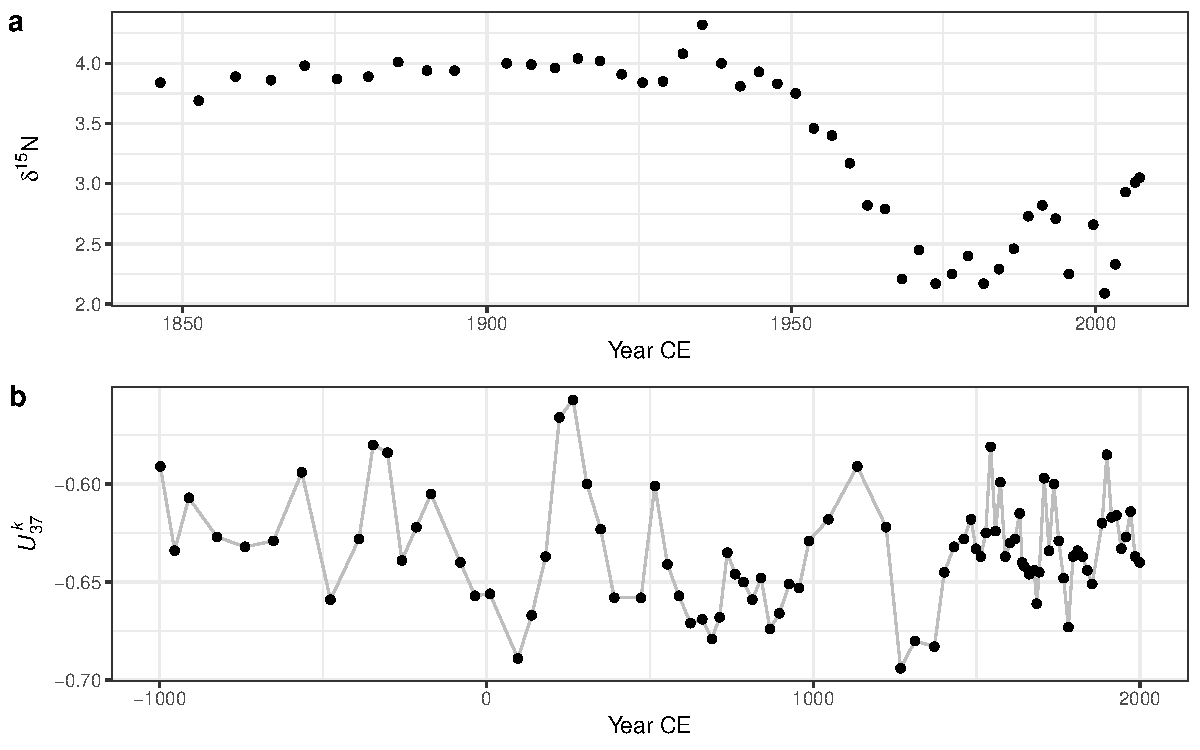
\includegraphics[width=0.8\linewidth]{supplementary-materials_files/figure-latex/data-figure-1} \end{center}

\section{Fitting GAMs}\label{fitting-gams}

The GAM plus CAR(1) process is fitted to the Small Water data set using
the \texttt{gamm()} function. This fits GAMs as mixed effects models via
the \emph{nlme} package, which allows the use of correlation structures
in the model residuals via the \texttt{correlation} argument. Here, the
\texttt{corCAR1()} function is used to select the CAR(1) process and we
specify the ordering of samples via the \texttt{Year} variable in
\texttt{small}.

\begin{Shaded}
\begin{Highlighting}[]
\NormalTok{## fit small water GAM usin gamm() with a CAR(1)}
\NormalTok{mod <-}\StringTok{ }\KeywordTok{gamm}\NormalTok{(d15N ~}\StringTok{ }\KeywordTok{s}\NormalTok{(Year, }\DataTypeTok{k =} \DecValTok{15}\NormalTok{), }\DataTypeTok{data =} \NormalTok{small,}
            \DataTypeTok{correlation =} \KeywordTok{corCAR1}\NormalTok{(}\DataTypeTok{form =} \NormalTok{~}\StringTok{ }\NormalTok{Year), }\DataTypeTok{method =} \StringTok{"REML"}\NormalTok{)}
\end{Highlighting}
\end{Shaded}

The estimated value of \(\phi\) for the CAR(1) can be extracted from the
fitted model via the \texttt{\$lme} component. Here we just extract the
correlation structure component.

\begin{Shaded}
\begin{Highlighting}[]
\NormalTok{## estimate of phi and confidence interval}
\NormalTok{smallPhi <-}\StringTok{ }\KeywordTok{intervals}\NormalTok{(mod$lme, }\DataTypeTok{which =} \StringTok{"var-cov"}\NormalTok{)$corStruct}
\NormalTok{smallPhi}
\end{Highlighting}
\end{Shaded}

\begin{verbatim}
#>         lower      est.     upper
#> Phi 0.2811107 0.6026967 0.8547543
#> attr(,"label")
#> [1] "Correlation structure:"
\end{verbatim}

The model summary is prepared from the \texttt{\$gam} component of the
fitted model

\begin{Shaded}
\begin{Highlighting}[]
\NormalTok{## summary object}
\KeywordTok{summary}\NormalTok{(mod$gam)}
\end{Highlighting}
\end{Shaded}

\begin{verbatim}
#> 
#> Family: gaussian 
#> Link function: identity 
#> 
#> Formula:
#> d15N ~ s(Year, k = 15)
#> 
#> Parametric coefficients:
#>             Estimate Std. Error t value Pr(>|t|)    
#> (Intercept)  3.30909    0.03489   94.84   <2e-16 ***
#> ---
#> Signif. codes:  0 '***' 0.001 '**' 0.01 '*' 0.05 '.' 0.1 ' ' 1
#> 
#> Approximate significance of smooth terms:
#>           edf Ref.df     F p-value    
#> s(Year) 7.954  7.954 47.44  <2e-16 ***
#> ---
#> Signif. codes:  0 '***' 0.001 '**' 0.01 '*' 0.05 '.' 0.1 ' ' 1
#> 
#> R-sq.(adj) =  0.929   
#>   Scale est. = 0.037268  n = 48
\end{verbatim}

The output shows the estimated complexity of the fitted smooth, in terms
of the effective degrees of freedom of the spline. An associated \(F\)
statistic and test of the null hypothesis of no trend (effect). Here the
estimated trend provides strong evidence against this null.

The CAR(1) process plotted in Figure 10 of the manuscript was prepared
using

\begin{Shaded}
\begin{Highlighting}[]
\NormalTok{## plot CAR(1) process}
\NormalTok{maxS <-}\StringTok{ }\KeywordTok{with}\NormalTok{(small, }\KeywordTok{diff}\NormalTok{(}\KeywordTok{range}\NormalTok{(Year))) ## too large, truncate to 50}
\NormalTok{S <-}\StringTok{ }\KeywordTok{seq}\NormalTok{(}\DecValTok{0}\NormalTok{, }\DecValTok{50}\NormalTok{, }\DataTypeTok{length =} \DecValTok{100}\NormalTok{)}

\NormalTok{car1 <-}\StringTok{ }\KeywordTok{setNames}\NormalTok{(}\KeywordTok{as.data.frame}\NormalTok{(}\KeywordTok{t}\NormalTok{(}\KeywordTok{outer}\NormalTok{(smallPhi, S, }\DataTypeTok{FUN =} \StringTok{`}\DataTypeTok{^}\StringTok{`}\NormalTok{)[}\DecValTok{1}\NormalTok{, , ])),}
                 \KeywordTok{c}\NormalTok{(}\StringTok{"Lower"}\NormalTok{,}\StringTok{"Correlation"}\NormalTok{,}\StringTok{"Upper"}\NormalTok{))}
\NormalTok{car1 <-}\StringTok{ }\KeywordTok{transform}\NormalTok{(car1, }\DataTypeTok{S =} \NormalTok{S)}

\NormalTok{car1Plt <-}\StringTok{ }\KeywordTok{ggplot}\NormalTok{(car1, }\KeywordTok{aes}\NormalTok{(}\DataTypeTok{x =} \NormalTok{S, }\DataTypeTok{y =} \NormalTok{Correlation)) +}
\StringTok{    }\KeywordTok{geom_ribbon}\NormalTok{(}\KeywordTok{aes}\NormalTok{(}\DataTypeTok{ymax =} \NormalTok{Upper, }\DataTypeTok{ymin =} \NormalTok{Lower),}
                \DataTypeTok{fill =} \StringTok{"black"}\NormalTok{, }\DataTypeTok{alpha =} \FloatTok{0.2}\NormalTok{) +}
\StringTok{    }\KeywordTok{geom_line}\NormalTok{() +}
\StringTok{    }\KeywordTok{ylab}\NormalTok{(}\KeywordTok{expression}\NormalTok{(}\KeywordTok{italic}\NormalTok{(h) *}\StringTok{ }\NormalTok{(}\KeywordTok{list}\NormalTok{(Delta[t], varphi)))) +}
\StringTok{    }\KeywordTok{xlab}\NormalTok{(}\KeywordTok{expression}\NormalTok{(Delta[t] ~}\StringTok{ }\NormalTok{(years)))}
\NormalTok{car1Plt}
\end{Highlighting}
\end{Shaded}

\begin{center}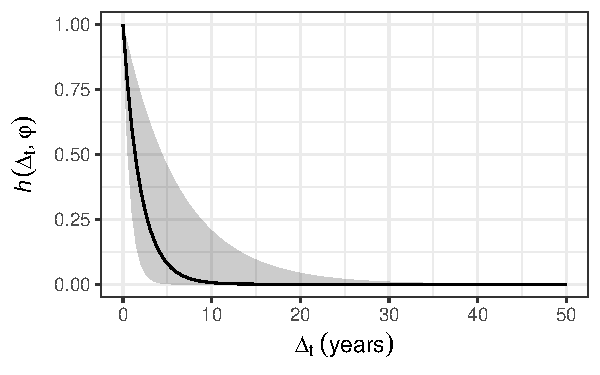
\includegraphics[width=0.8\linewidth]{supplementary-materials_files/figure-latex/car1-plot-1} \end{center}

The exponential decline in correlation with increasing separation is
evident here; once samples are \textasciitilde{}10 years apart, there is
little estimated dependence between them.

The same model is fitted to the Braya-Sø data set. Note however that in
order to even fit the model with both a smooth and the CAR(1) process, I
have had to change the default optimiser used to fit the model, and
reduce the basis dimension to a small number. We also fit the model
using GCV, which is the defaut, hence no \texttt{method} argument

\begin{Shaded}
\begin{Highlighting}[]
\NormalTok{## fit the car(1) model --- needs optim as this is not a stable fit!}
\NormalTok{## also needs k setting lower than default}
\NormalTok{braya.car1 <-}\StringTok{ }\KeywordTok{gamm}\NormalTok{(UK37 ~}\StringTok{ }\KeywordTok{s}\NormalTok{(Year, }\DataTypeTok{k =} \DecValTok{5}\NormalTok{), }\DataTypeTok{data =} \NormalTok{braya, }
                   \DataTypeTok{correlation =} \KeywordTok{corCAR1}\NormalTok{(}\DataTypeTok{form =} \NormalTok{~}\StringTok{ }\NormalTok{Year),}
                   \DataTypeTok{method =} \StringTok{"REML"}\NormalTok{,}
                   \DataTypeTok{control =} \KeywordTok{list}\NormalTok{(}\DataTypeTok{niterEM =} \DecValTok{0}\NormalTok{, }\DataTypeTok{optimMethod =} \StringTok{"BFGS"}\NormalTok{, }
                                  \DataTypeTok{opt =} \StringTok{"optim"}\NormalTok{))}

\NormalTok{## fit model using GCV}
\NormalTok{braya.gcv <-}\StringTok{ }\KeywordTok{gam}\NormalTok{(UK37 ~}\StringTok{ }\KeywordTok{s}\NormalTok{(Year, }\DataTypeTok{k =} \DecValTok{30}\NormalTok{), }\DataTypeTok{data =} \NormalTok{braya)}

\NormalTok{## estimate of phi and confidence interval}
\NormalTok{brayaPhi <-}\StringTok{ }\KeywordTok{intervals}\NormalTok{(braya.car1$lme)$corStruct}
\NormalTok{brayaPhi}
\end{Highlighting}
\end{Shaded}

\begin{verbatim}
#>            lower      est. upper
#> Phi 1.611049e-22 0.2000156     1
#> attr(,"label")
#> [1] "Correlation structure:"
\end{verbatim}

Note the wide confidence interval --- effectively 0--1 --- on \(\phi\).
If you were to increase the value of \texttt{k} to be \texttt{k\ =\ 10}
in the \texttt{s(Year)} above, the model will fit but a warning message
will be emitted when trying to extract \(\phi\) due to a non-positive
definite model covariance matrix, indicating problems with the model.

The next couple of code chunks prepare plots of the fitted GAMS. The
general idea is to predict fom the fitted model for a fine grid of
points over the range of the time variable. First we plot the trend for
Small Water with an approximate 95\% confidence interval assuming
asymptotic normality

\begin{Shaded}
\begin{Highlighting}[]
\NormalTok{N <-}\StringTok{ }\DecValTok{300}   \CommentTok{# number of points at which to evaluate the splines}
\NormalTok{## Predict from the fitted model}
\NormalTok{newYear <-}\StringTok{ }\KeywordTok{with}\NormalTok{(small, }\KeywordTok{data.frame}\NormalTok{(}\DataTypeTok{Year =} \KeywordTok{seq}\NormalTok{(}\KeywordTok{min}\NormalTok{(Year), }\KeywordTok{max}\NormalTok{(Year),}
                                             \DataTypeTok{length.out =} \DecValTok{200}\NormalTok{)))}
\NormalTok{newYear <-}\StringTok{ }\KeywordTok{cbind}\NormalTok{(newYear,}
                 \KeywordTok{data.frame}\NormalTok{(}\KeywordTok{predict}\NormalTok{(mod$gam, newYear, }\DataTypeTok{se.fit =} \OtherTok{TRUE}\NormalTok{)))}
\NormalTok{newYear <-}\StringTok{ }\KeywordTok{transform}\NormalTok{(newYear,}
                     \DataTypeTok{upper =} \NormalTok{fit +}\StringTok{ }\NormalTok{(}\DecValTok{2} \NormalTok{*}\StringTok{ }\NormalTok{se.fit),}
                     \DataTypeTok{lower =} \NormalTok{fit -}\StringTok{ }\NormalTok{(}\DecValTok{2} \NormalTok{*}\StringTok{ }\NormalTok{se.fit))}

\NormalTok{## Plot simulated trends}
\NormalTok{small_fitted <-}\StringTok{ }\KeywordTok{ggplot}\NormalTok{(newYear, }\KeywordTok{aes}\NormalTok{(}\DataTypeTok{x =} \NormalTok{Year, }\DataTypeTok{y =} \NormalTok{fit)) +}
\StringTok{    }\KeywordTok{geom_ribbon}\NormalTok{(}\KeywordTok{aes}\NormalTok{(}\DataTypeTok{ymin =} \NormalTok{lower, }\DataTypeTok{ymax =} \NormalTok{upper, }\DataTypeTok{x =} \NormalTok{Year), }\DataTypeTok{alpha =} \FloatTok{0.2}\NormalTok{,}
                \DataTypeTok{inherit.aes =} \OtherTok{FALSE}\NormalTok{, }\DataTypeTok{fill =} \StringTok{"black"}\NormalTok{) +}
\StringTok{    }\KeywordTok{geom_point}\NormalTok{(}\DataTypeTok{data =} \NormalTok{small, }\DataTypeTok{mapping =} \KeywordTok{aes}\NormalTok{(}\DataTypeTok{x =} \NormalTok{Year, }\DataTypeTok{y =} \NormalTok{d15N),}
               \DataTypeTok{inherit.aes =} \OtherTok{FALSE}\NormalTok{) +}
\StringTok{    }\KeywordTok{geom_line}\NormalTok{() +}
\StringTok{    }\KeywordTok{labs}\NormalTok{(}\DataTypeTok{y =} \NormalTok{d15n_label, }\DataTypeTok{x =} \StringTok{"Year CE"}\NormalTok{)}
\NormalTok{small_fitted}
\end{Highlighting}
\end{Shaded}

\begin{center}\includegraphics[width=0.8\linewidth]{supplementary-materials_files/figure-latex/small-plot-fitted-models-1} \end{center}

For Braya-Sø, we repeat the process, but we do so for both models (GAMM
+ CAR(1) and GCV), and use a critical value from the \(t\) distribution
to form the confidence interval

\begin{Shaded}
\begin{Highlighting}[]
\NormalTok{## ggplot with data and fitted spline, then resids vs time in second panel}
\NormalTok{newBraya <-}\StringTok{ }\KeywordTok{with}\NormalTok{(braya, }\KeywordTok{data.frame}\NormalTok{(}\DataTypeTok{Year =} \KeywordTok{seq}\NormalTok{(}\KeywordTok{min}\NormalTok{(Year), }\KeywordTok{max}\NormalTok{(Year),}
                                              \DataTypeTok{length.out =} \NormalTok{N)))}
\NormalTok{newBraya <-}\StringTok{ }\KeywordTok{cbind}\NormalTok{(newBraya,}
                  \KeywordTok{data.frame}\NormalTok{(}\KeywordTok{predict}\NormalTok{(braya.car1$gam, newBraya,}
                                     \DataTypeTok{se.fit =} \OtherTok{TRUE}\NormalTok{)))}
\NormalTok{crit.t <-}\StringTok{ }\KeywordTok{qt}\NormalTok{(}\FloatTok{0.975}\NormalTok{, }\DataTypeTok{df =} \KeywordTok{df.residual}\NormalTok{(braya.car1$gam))}
\NormalTok{newBraya <-}\StringTok{ }\KeywordTok{transform}\NormalTok{(newBraya,}
                      \DataTypeTok{upper =} \NormalTok{fit +}\StringTok{ }\NormalTok{(crit.t *}\StringTok{ }\NormalTok{se.fit),}
                      \DataTypeTok{lower =} \NormalTok{fit -}\StringTok{ }\NormalTok{(crit.t *}\StringTok{ }\NormalTok{se.fit))}
\NormalTok{## add GAM GCV results}
\NormalTok{fit_gcv <-}\StringTok{ }\KeywordTok{predict}\NormalTok{(braya.gcv, }\DataTypeTok{newdata =} \NormalTok{newBraya, }\DataTypeTok{se.fit =} \OtherTok{TRUE}\NormalTok{)}
\NormalTok{newBraya <-}\StringTok{ }\KeywordTok{rbind}\NormalTok{(newBraya, newBraya) }\CommentTok{# extend newBraya to take GCV results}
\NormalTok{newBraya[}\KeywordTok{seq}\NormalTok{(N}\DecValTok{+1}\NormalTok{, }\DataTypeTok{length.out =} \NormalTok{N, }\DataTypeTok{by =} \DecValTok{1}\NormalTok{), ]$fit <-}\StringTok{ }\NormalTok{fit_gcv$fit}
\NormalTok{newBraya[}\KeywordTok{seq}\NormalTok{(N}\DecValTok{+1}\NormalTok{, }\DataTypeTok{length.out =} \NormalTok{N, }\DataTypeTok{by =} \DecValTok{1}\NormalTok{), ]$upper <-}
\StringTok{    }\NormalTok{fit_gcv$fit +}\StringTok{ }\NormalTok{(}\KeywordTok{qt}\NormalTok{(}\FloatTok{0.975}\NormalTok{, }\KeywordTok{df.residual}\NormalTok{(braya.gcv)) *}\StringTok{ }\NormalTok{fit_gcv$se.fit)}
\NormalTok{newBraya[}\KeywordTok{seq}\NormalTok{(N}\DecValTok{+1}\NormalTok{, }\DataTypeTok{length.out =} \NormalTok{N, }\DataTypeTok{by =} \DecValTok{1}\NormalTok{), ]$lower <-}
\StringTok{    }\NormalTok{fit_gcv$fit -}\StringTok{ }\NormalTok{(}\KeywordTok{qt}\NormalTok{(}\FloatTok{0.975}\NormalTok{, }\KeywordTok{df.residual}\NormalTok{(braya.gcv)) *}\StringTok{ }\NormalTok{fit_gcv$se.fit)}
\NormalTok{newBraya <-}\StringTok{ }\KeywordTok{transform}\NormalTok{(newBraya,}
                      \DataTypeTok{Method =} \KeywordTok{rep}\NormalTok{(}\KeywordTok{c}\NormalTok{(}\StringTok{"GAMM (CAR(1))"}\NormalTok{, }\StringTok{"GAM (GCV)"}\NormalTok{), }
                                   \DataTypeTok{each =} \NormalTok{N))}

\NormalTok{## plot CAR(1) and GCV fits}
\NormalTok{braya_fitted <-}\StringTok{ }\KeywordTok{ggplot}\NormalTok{(braya, }\KeywordTok{aes}\NormalTok{(}\DataTypeTok{y =} \NormalTok{UK37, }\DataTypeTok{x =} \NormalTok{Year)) +}
\StringTok{    }\KeywordTok{geom_point}\NormalTok{() +}
\StringTok{    }\KeywordTok{geom_ribbon}\NormalTok{(}\DataTypeTok{data =} \NormalTok{newBraya,}
                \DataTypeTok{mapping =} \KeywordTok{aes}\NormalTok{(}\DataTypeTok{x =} \NormalTok{Year, }\DataTypeTok{ymax =} \NormalTok{upper, }\DataTypeTok{ymin =} \NormalTok{lower,}
                              \DataTypeTok{fill =} \NormalTok{Method),}
                \DataTypeTok{alpha =} \FloatTok{0.3}\NormalTok{, }\DataTypeTok{inherit.aes =} \OtherTok{FALSE}\NormalTok{) +}
\StringTok{    }\KeywordTok{geom_line}\NormalTok{(}\DataTypeTok{data =} \NormalTok{newBraya,}
              \DataTypeTok{mapping =} \KeywordTok{aes}\NormalTok{(}\DataTypeTok{y =} \NormalTok{fit, }\DataTypeTok{x =} \NormalTok{Year, }\DataTypeTok{colour =} \NormalTok{Method)) +}
\StringTok{    }\KeywordTok{labs}\NormalTok{(}\DataTypeTok{y =} \NormalTok{braya_ylabel, }\DataTypeTok{x =} \StringTok{"Year CE"}\NormalTok{) +}
\StringTok{    }\KeywordTok{scale_color_manual}\NormalTok{(}\DataTypeTok{values =} \KeywordTok{c}\NormalTok{(}\StringTok{"#5e3c99"}\NormalTok{, }\StringTok{"#e66101"}\NormalTok{)) +}
\StringTok{    }\KeywordTok{scale_fill_manual}\NormalTok{(}\DataTypeTok{values =} \KeywordTok{c}\NormalTok{(}\StringTok{"#5e3c99"}\NormalTok{, }\StringTok{"#e66101"}\NormalTok{)) +}
\StringTok{    }\KeywordTok{theme}\NormalTok{(}\DataTypeTok{legend.position =} \StringTok{"right"}\NormalTok{)}
\NormalTok{braya_fitted}
\end{Highlighting}
\end{Shaded}

\begin{center}\includegraphics[width=0.8\linewidth]{supplementary-materials_files/figure-latex/braya-plot-fitted-models-1} \end{center}

Figure 5 in the manuscript was produced using:

\begin{Shaded}
\begin{Highlighting}[]
\KeywordTok{plot_grid}\NormalTok{(small_fitted, braya_fitted, }\DataTypeTok{ncol =} \DecValTok{1}\NormalTok{, }\DataTypeTok{labels =} \StringTok{"auto"}\NormalTok{,}
          \DataTypeTok{align =} \StringTok{"hv"}\NormalTok{, }\DataTypeTok{axis =} \StringTok{"lr"}\NormalTok{)}
\end{Highlighting}
\end{Shaded}

\begin{center}\includegraphics[width=0.8\linewidth]{supplementary-materials_files/figure-latex/manuscript-fig-2-1} \end{center}

To proceed with the Braya-Sø example, we need to increase the basis
dimension (\texttt{k\ =\ 45}), fit using \texttt{method\ =\ "REML"}, and
use observational weights. Here I use the \texttt{sampleInterval}
variable as the measure of lake years per sample, and to avoid changing
the model likelihood, the weights are actually the values of
\texttt{sampleInterval} divided by the mean of \texttt{sampleInterval}:

\begin{Shaded}
\begin{Highlighting}[]
\NormalTok{## TPRS, weights as sampleInterval}
\NormalTok{braya_reml <-}\StringTok{ }\KeywordTok{gam}\NormalTok{(UK37 ~}\StringTok{ }\KeywordTok{s}\NormalTok{(Year, }\DataTypeTok{k =} \DecValTok{45}\NormalTok{, }\DataTypeTok{bs =} \StringTok{"tp"}\NormalTok{), }\DataTypeTok{data =} \NormalTok{braya,}
                  \DataTypeTok{method =} \StringTok{"REML"}\NormalTok{,}
                  \DataTypeTok{weights =} \NormalTok{sampleInterval /}\StringTok{ }\KeywordTok{mean}\NormalTok{(sampleInterval))}
\end{Highlighting}
\end{Shaded}

\section{Posterior simulation}\label{posterior-simulation}

Samples from the posterior distribution of a GAM can be drawn using the
\texttt{simulate()} methods from the \emph{schoenberg} package.

\begin{Shaded}
\begin{Highlighting}[]
\KeywordTok{set.seed}\NormalTok{(}\DecValTok{1}\NormalTok{) }\CommentTok{# set the random seed to make this reproducible}
\NormalTok{nsim <-}\StringTok{ }\DecValTok{20}  \CommentTok{# how many simulations to draw}

\NormalTok{## do the simulations}
\NormalTok{sims <-}\StringTok{ }\KeywordTok{simulate}\NormalTok{(mod, }\DataTypeTok{nsim =} \NormalTok{nsim, }\DataTypeTok{newdata =} \NormalTok{newYear, }\DataTypeTok{unconditional =} \OtherTok{TRUE}\NormalTok{)}

\NormalTok{## rearrange the output into a long/tidy format}
\KeywordTok{colnames}\NormalTok{(sims) <-}\StringTok{ }\KeywordTok{paste0}\NormalTok{(}\StringTok{"sim"}\NormalTok{, }\KeywordTok{seq_len}\NormalTok{(nsim))}
\NormalTok{sims <-}\StringTok{ }\KeywordTok{setNames}\NormalTok{(}\KeywordTok{stack}\NormalTok{(}\KeywordTok{as.data.frame}\NormalTok{(sims)), }\KeywordTok{c}\NormalTok{(}\StringTok{"simulated"}\NormalTok{, }\StringTok{"run"}\NormalTok{))}
\NormalTok{sims <-}\StringTok{ }\KeywordTok{transform}\NormalTok{(sims, }\DataTypeTok{Year =} \KeywordTok{rep}\NormalTok{(newYear$Year, nsim),}
                  \DataTypeTok{simulated =} \NormalTok{simulated)}

\NormalTok{## Plot simulated trends}
\NormalTok{smallSim.plt <-}\StringTok{ }\KeywordTok{ggplot}\NormalTok{(newYear, }\KeywordTok{aes}\NormalTok{(}\DataTypeTok{x =} \NormalTok{Year, }\DataTypeTok{y =} \NormalTok{fit)) +}
\StringTok{    }\KeywordTok{geom_line}\NormalTok{(}\DataTypeTok{data =} \NormalTok{sims,}
              \DataTypeTok{mapping =} \KeywordTok{aes}\NormalTok{(}\DataTypeTok{y =} \NormalTok{simulated, }\DataTypeTok{x =} \NormalTok{Year, }\DataTypeTok{group =} \NormalTok{run),}
              \DataTypeTok{colour =} \StringTok{"grey80"}\NormalTok{) +}
\StringTok{    }\KeywordTok{geom_line}\NormalTok{(}\DataTypeTok{lwd =} \DecValTok{1}\NormalTok{) +}
\StringTok{    }\KeywordTok{labs}\NormalTok{(}\DataTypeTok{y =} \NormalTok{d15n_label, }\DataTypeTok{x =} \StringTok{"Year CE"}\NormalTok{)}
\NormalTok{smallSim.plt}
\end{Highlighting}
\end{Shaded}

\begin{center}\includegraphics[width=0.8\linewidth]{supplementary-materials_files/figure-latex/small-posterior-simulation-1} \end{center}

We repeat the same simulation for Braya-Sø

\begin{Shaded}
\begin{Highlighting}[]
\NormalTok{## posterior simulation}
\NormalTok{## need to reset-up newBraya}
\NormalTok{newBraya <-}\StringTok{ }\KeywordTok{with}\NormalTok{(braya,}
                 \KeywordTok{data.frame}\NormalTok{(}\DataTypeTok{Year =} \KeywordTok{seq}\NormalTok{(}\KeywordTok{min}\NormalTok{(Year), }\KeywordTok{max}\NormalTok{(Year),}
                                       \DataTypeTok{length.out =} \NormalTok{N)))}
\NormalTok{braya_pred <-}\StringTok{ }\KeywordTok{cbind}\NormalTok{(newBraya,}
                    \KeywordTok{data.frame}\NormalTok{(}\KeywordTok{predict}\NormalTok{(braya_reml, newBraya,}
                                       \DataTypeTok{se.fit =} \OtherTok{TRUE}\NormalTok{)))}

\NormalTok{## simulate}
\KeywordTok{set.seed}\NormalTok{(}\DecValTok{1}\NormalTok{)}
\NormalTok{sims2 <-}\StringTok{ }\KeywordTok{simulate}\NormalTok{(braya_reml, }\DataTypeTok{nsim =} \NormalTok{nsim, }\DataTypeTok{newdata =} \NormalTok{newBraya,}
                  \DataTypeTok{unconditional =} \OtherTok{TRUE}\NormalTok{)}
\KeywordTok{colnames}\NormalTok{(sims2) <-}\StringTok{ }\KeywordTok{paste0}\NormalTok{(}\StringTok{"sim"}\NormalTok{, }\KeywordTok{seq_len}\NormalTok{(nsim))}
\NormalTok{sims2 <-}\StringTok{ }\KeywordTok{setNames}\NormalTok{(}\KeywordTok{stack}\NormalTok{(}\KeywordTok{as.data.frame}\NormalTok{(sims2)),}
                      \KeywordTok{c}\NormalTok{(}\StringTok{"simulated"}\NormalTok{, }\StringTok{"run"}\NormalTok{))}
\NormalTok{sims2 <-}\StringTok{ }\KeywordTok{transform}\NormalTok{(sims2, }\DataTypeTok{Year =} \KeywordTok{rep}\NormalTok{(newBraya$Year, nsim),}
                       \DataTypeTok{simulated =} \NormalTok{simulated)}

\NormalTok{brayaSim.plt <-}\StringTok{ }\KeywordTok{ggplot}\NormalTok{(braya_pred, }\KeywordTok{aes}\NormalTok{(}\DataTypeTok{x =} \NormalTok{Year, }\DataTypeTok{y =} \NormalTok{fit)) +}
\StringTok{    }\KeywordTok{geom_line}\NormalTok{(}\DataTypeTok{data =} \NormalTok{sims2,}
              \DataTypeTok{mapping =} \KeywordTok{aes}\NormalTok{(}\DataTypeTok{y =} \NormalTok{simulated, }\DataTypeTok{x =} \NormalTok{Year, }\DataTypeTok{group =} \NormalTok{run),}
              \DataTypeTok{colour =} \StringTok{"grey80"}\NormalTok{) +}
\StringTok{    }\KeywordTok{geom_line}\NormalTok{(}\DataTypeTok{lwd =} \DecValTok{1}\NormalTok{) +}
\StringTok{    }\KeywordTok{labs}\NormalTok{(}\DataTypeTok{y =} \NormalTok{braya_ylabel, }\DataTypeTok{x =} \StringTok{"Year CE"}\NormalTok{)}
\NormalTok{brayaSim.plt}
\end{Highlighting}
\end{Shaded}

\begin{center}\includegraphics[width=0.8\linewidth]{supplementary-materials_files/figure-latex/braya-posterior-simulation-1} \end{center}

Figure 7 in the manuscript was prepared using

\begin{Shaded}
\begin{Highlighting}[]
\KeywordTok{plot_grid}\NormalTok{(smallSim.plt, brayaSim.plt, }\DataTypeTok{ncol =} \DecValTok{1}\NormalTok{, }\DataTypeTok{labels =} \StringTok{"auto"}\NormalTok{,}
          \DataTypeTok{align =} \StringTok{"hv"}\NormalTok{, }\DataTypeTok{axis =} \StringTok{"lr"}\NormalTok{)}
\end{Highlighting}
\end{Shaded}

\begin{center}\includegraphics[width=0.8\linewidth]{supplementary-materials_files/figure-latex/figure-7-1} \end{center}

\section{Confidence and simultaneous
intervals}\label{confidence-and-simultaneous-intervals}

Across-the-function and simultaneous confidence intervals are computed
using the \texttt{confint()} method. The type of interval required is
given via the \texttt{type} argument with options \texttt{"confidence"}
and \texttt{"simultaneous"}.

\begin{Shaded}
\begin{Highlighting}[]
\NormalTok{## small water}
\NormalTok{sw.cint <-}\StringTok{ }\KeywordTok{confint}\NormalTok{(mod, }\DataTypeTok{parm =} \StringTok{"Year"}\NormalTok{, }\DataTypeTok{newdata =} \NormalTok{newYear,}
                   \DataTypeTok{type =} \StringTok{"confidence"}\NormalTok{)}
\NormalTok{sw.sint <-}\StringTok{ }\KeywordTok{confint}\NormalTok{(mod, }\DataTypeTok{parm =} \StringTok{"Year"}\NormalTok{, }\DataTypeTok{newdata =} \NormalTok{newYear,}
                   \DataTypeTok{type =} \StringTok{"simultaneous"}\NormalTok{)}

\NormalTok{smallInt.plt <-}\StringTok{ }\KeywordTok{ggplot}\NormalTok{(sw.cint, }\KeywordTok{aes}\NormalTok{(}\DataTypeTok{x =} \NormalTok{Year, }\DataTypeTok{y =} \NormalTok{est)) +}
\StringTok{    }\KeywordTok{geom_ribbon}\NormalTok{(}\DataTypeTok{data =} \NormalTok{sw.sint,}
                \DataTypeTok{mapping =} \KeywordTok{aes}\NormalTok{(}\DataTypeTok{ymin =} \NormalTok{lower, }\DataTypeTok{ymax =} \NormalTok{upper, }\DataTypeTok{x =} \NormalTok{Year),}
                \DataTypeTok{fill =} \StringTok{"grey80"}\NormalTok{, }\DataTypeTok{inherit.aes =} \OtherTok{FALSE}\NormalTok{) +}
\StringTok{    }\KeywordTok{geom_ribbon}\NormalTok{(}\DataTypeTok{mapping =} \KeywordTok{aes}\NormalTok{(}\DataTypeTok{ymin =} \NormalTok{lower, }\DataTypeTok{ymax =} \NormalTok{upper, }\DataTypeTok{x =} \NormalTok{Year),}
                \DataTypeTok{fill =} \StringTok{"grey60"}\NormalTok{, }\DataTypeTok{inherit.aes =} \OtherTok{FALSE}\NormalTok{) +}
\StringTok{    }\KeywordTok{geom_line}\NormalTok{(}\DataTypeTok{lwd =} \DecValTok{1}\NormalTok{) +}
\StringTok{    }\KeywordTok{labs}\NormalTok{(}\DataTypeTok{y =} \NormalTok{d15n_label, }\DataTypeTok{x =} \StringTok{"Year CE"}\NormalTok{)}
\NormalTok{smallInt.plt}
\end{Highlighting}
\end{Shaded}

\begin{center}\includegraphics[width=0.8\linewidth]{supplementary-materials_files/figure-latex/small-compare-intervals-1} \end{center}

\begin{Shaded}
\begin{Highlighting}[]
\NormalTok{## braya so}
\NormalTok{bs.cint <-}\StringTok{ }\KeywordTok{confint}\NormalTok{(braya_reml, }\DataTypeTok{parm =} \StringTok{"Year"}\NormalTok{, }\DataTypeTok{newdata =} \NormalTok{newBraya,}
                   \DataTypeTok{type =} \StringTok{"confidence"}\NormalTok{)}
\NormalTok{bs.sint <-}\StringTok{ }\KeywordTok{confint}\NormalTok{(braya_reml, }\DataTypeTok{parm =} \StringTok{"Year"}\NormalTok{, }\DataTypeTok{newdata =} \NormalTok{newBraya,}
                   \DataTypeTok{type =} \StringTok{"simultaneous"}\NormalTok{)}

\NormalTok{brayaInt.plt <-}\StringTok{ }\KeywordTok{ggplot}\NormalTok{(bs.cint, }\KeywordTok{aes}\NormalTok{(}\DataTypeTok{x =} \NormalTok{Year, }\DataTypeTok{y =} \NormalTok{est)) +}
\StringTok{    }\KeywordTok{geom_ribbon}\NormalTok{(}\DataTypeTok{data =} \NormalTok{bs.sint,}
                \DataTypeTok{mapping =} \KeywordTok{aes}\NormalTok{(}\DataTypeTok{ymin =} \NormalTok{lower, }\DataTypeTok{ymax =} \NormalTok{upper, }\DataTypeTok{x =} \NormalTok{Year),}
                \DataTypeTok{fill =} \StringTok{"grey80"}\NormalTok{, }\DataTypeTok{inherit.aes =} \OtherTok{FALSE}\NormalTok{) +}
\StringTok{    }\KeywordTok{geom_ribbon}\NormalTok{(}\DataTypeTok{mapping =} \KeywordTok{aes}\NormalTok{(}\DataTypeTok{ymin =} \NormalTok{lower, }\DataTypeTok{ymax =} \NormalTok{upper, }\DataTypeTok{x =} \NormalTok{Year),}
                \DataTypeTok{fill =} \StringTok{"grey60"}\NormalTok{, }\DataTypeTok{inherit.aes =} \OtherTok{FALSE}\NormalTok{) +}
\StringTok{    }\KeywordTok{geom_line}\NormalTok{(}\DataTypeTok{lwd =} \DecValTok{1}\NormalTok{) +}
\StringTok{    }\KeywordTok{labs}\NormalTok{(}\DataTypeTok{y =} \NormalTok{braya_ylabel, }\DataTypeTok{x =} \StringTok{"Year CE"}\NormalTok{)}
\NormalTok{brayaInt.plt}
\end{Highlighting}
\end{Shaded}

\begin{center}\includegraphics[width=0.8\linewidth]{supplementary-materials_files/figure-latex/braya-compare-intervals-1} \end{center}

Figure 8 in the manuscript was prepared using

\begin{Shaded}
\begin{Highlighting}[]
\KeywordTok{plot_grid}\NormalTok{(smallInt.plt, brayaInt.plt, }\DataTypeTok{ncol =} \DecValTok{1}\NormalTok{, }\DataTypeTok{labels =} \StringTok{"auto"}\NormalTok{,}
          \DataTypeTok{align =} \StringTok{"hv"}\NormalTok{, }\DataTypeTok{axis =} \StringTok{"lr"}\NormalTok{)}
\end{Highlighting}
\end{Shaded}

\begin{center}\includegraphics[width=0.8\linewidth]{supplementary-materials_files/figure-latex/figure-8-1} \end{center}

\section{Derivatives of the estimated
trend}\label{derivatives-of-the-estimated-trend}

The first derivative of the estimated trend is calculated using finite
differences using the \texttt{fderiv()} function. There is also a
\texttt{confint()} method for objects produced by \texttt{fderiv()}. The
first derivatives and a 95\% simultaneous confidence interval for the
Small Water trend we computed and plotted using

\begin{Shaded}
\begin{Highlighting}[]
\NormalTok{small.d <-}\StringTok{ }\KeywordTok{fderiv}\NormalTok{(mod, }\DataTypeTok{newdata =} \NormalTok{newYear, }\DataTypeTok{n =} \NormalTok{N)}
\NormalTok{small.sint <-}\StringTok{ }\KeywordTok{with}\NormalTok{(newYear,}
                   \KeywordTok{cbind}\NormalTok{(}\KeywordTok{confint}\NormalTok{(small.d, }\DataTypeTok{nsim =} \NormalTok{nsim,}
                                 \DataTypeTok{type =} \StringTok{"simultaneous"}\NormalTok{),}
                         \DataTypeTok{Year =} \NormalTok{Year))}

\NormalTok{small_deriv_plt <-}\StringTok{ }\KeywordTok{ggplot}\NormalTok{(small.sint, }\KeywordTok{aes}\NormalTok{(}\DataTypeTok{x =} \NormalTok{Year, }\DataTypeTok{y =} \NormalTok{est)) +}
\StringTok{    }\KeywordTok{geom_ribbon}\NormalTok{(}\KeywordTok{aes}\NormalTok{(}\DataTypeTok{ymin =} \NormalTok{lower, }\DataTypeTok{ymax =} \NormalTok{upper), }\DataTypeTok{alpha =} \FloatTok{0.2}\NormalTok{,}
                \DataTypeTok{fill =} \StringTok{"black"}\NormalTok{) +}
\StringTok{    }\KeywordTok{geom_line}\NormalTok{() +}
\StringTok{    }\KeywordTok{labs}\NormalTok{(}\DataTypeTok{x =} \StringTok{"Year CE"}\NormalTok{, }\DataTypeTok{y =} \StringTok{"First derivative"}\NormalTok{)}
\end{Highlighting}
\end{Shaded}

whilst for Braya-Sø, the following was used

\begin{Shaded}
\begin{Highlighting}[]
\NormalTok{braya.d <-}\StringTok{ }\KeywordTok{fderiv}\NormalTok{(braya_reml, }\DataTypeTok{newdata =} \NormalTok{newBraya, }\DataTypeTok{n =} \NormalTok{N)}
\NormalTok{braya.sint <-}\StringTok{ }\KeywordTok{with}\NormalTok{(newBraya,}
                   \KeywordTok{cbind}\NormalTok{(}\KeywordTok{confint}\NormalTok{(braya.d, }\DataTypeTok{nsim =} \NormalTok{nsim,}
                                 \DataTypeTok{type =} \StringTok{"simultaneous"}\NormalTok{),}
                         \DataTypeTok{Year =} \NormalTok{Year))}

\NormalTok{braya_deriv_plt <-}\StringTok{ }\KeywordTok{ggplot}\NormalTok{(braya.sint, }\KeywordTok{aes}\NormalTok{(}\DataTypeTok{x =} \NormalTok{Year, }\DataTypeTok{y =} \NormalTok{est)) +}
\StringTok{    }\KeywordTok{geom_ribbon}\NormalTok{(}\KeywordTok{aes}\NormalTok{(}\DataTypeTok{ymin =} \NormalTok{lower, }\DataTypeTok{ymax =} \NormalTok{upper),}
                \DataTypeTok{alpha =} \FloatTok{0.2}\NormalTok{, }\DataTypeTok{fill =} \StringTok{"black"}\NormalTok{) +}
\StringTok{    }\KeywordTok{geom_line}\NormalTok{() +}
\StringTok{    }\KeywordTok{labs}\NormalTok{(}\DataTypeTok{x =} \StringTok{"Year CE"}\NormalTok{, }\DataTypeTok{y =} \StringTok{"First derivative"}\NormalTok{)}
\end{Highlighting}
\end{Shaded}

Figure 9 in the manuscript was prepared using

\begin{Shaded}
\begin{Highlighting}[]
\KeywordTok{plot_grid}\NormalTok{(small_deriv_plt, braya_deriv_plt, }\DataTypeTok{ncol =} \DecValTok{1}\NormalTok{, }\DataTypeTok{labels =} \StringTok{"auto"}\NormalTok{,}
          \DataTypeTok{align =} \StringTok{"hv"}\NormalTok{, }\DataTypeTok{axis =} \StringTok{"lr"}\NormalTok{)}
\end{Highlighting}
\end{Shaded}

\begin{center}\includegraphics[width=0.8\linewidth]{supplementary-materials_files/figure-latex/figure 9-1} \end{center}

\section{Gaussian process smooths}\label{gaussian-process-smooths}

For the Gaussian process smooth to fit within the GAM framework
described in the manuscript, we need to supply the value of \(\phi\) for
the effective range of the correlation function. To estimate \(\phi\),
we need to repeatedly fit the required GAM using a range of plausible
values for \(\phi\), which we do using a loop. In the chunk below I fit
200 models with \(\phi\) in the range 15--500. For value of \(\phi\) I
fit the required GAM and extract the REML score (from component
\texttt{gcv.ubre}) and store it in the numeric vectors \texttt{Mat} or
\texttt{SEx}, for Matérn and Squared Exponential correlation functions,
respectively. The final line of the chunk prepares the REML scores for
the two correlation functions in long or tidy format suitable for
plotting with \emph{ggplot2}.

\begin{Shaded}
\begin{Highlighting}[]
\NormalTok{nn <-}\StringTok{ }\DecValTok{200}    \CommentTok{# number of points at which to evaluate profile likelihood}
\NormalTok{dseq <-}\StringTok{ }\KeywordTok{seq}\NormalTok{(}\DecValTok{15}\NormalTok{, }\DecValTok{500}\NormalTok{, }\DataTypeTok{length.out =} \NormalTok{nn)  }\CommentTok{# effective ranges to fit at}
\NormalTok{Mat <-}\StringTok{ }\NormalTok{SEx <-}\StringTok{ }\KeywordTok{numeric}\NormalTok{(}\DataTypeTok{length =} \NormalTok{nn)     }\CommentTok{# object to hold model fits}
\NormalTok{for (i in }\KeywordTok{seq_along}\NormalTok{(dseq)) \{ }
    \NormalTok{## iterate over dseq, fit GP GAM w Matérn covariance}
    \NormalTok{Mat[i] <-}\StringTok{ }\KeywordTok{gam}\NormalTok{(UK37 ~}\StringTok{ }\KeywordTok{s}\NormalTok{(Year, }\DataTypeTok{k =} \DecValTok{45}\NormalTok{, }\DataTypeTok{bs =} \StringTok{"gp"}\NormalTok{, }\DataTypeTok{m =} \KeywordTok{c}\NormalTok{(}\DecValTok{3}\NormalTok{, dseq[i])),}
                  \DataTypeTok{weights =} \NormalTok{sampleInterval /}\StringTok{ }\KeywordTok{mean}\NormalTok{(sampleInterval),}
                  \DataTypeTok{data =} \NormalTok{braya, }\DataTypeTok{method =} \StringTok{"REML"}\NormalTok{,}
                  \DataTypeTok{family =} \KeywordTok{gaussian}\NormalTok{())[[}\StringTok{"gcv.ubre"}\NormalTok{]]}
    \NormalTok{## fit squared exponential}
    \NormalTok{SEx[i] <-}\StringTok{ }\KeywordTok{gam}\NormalTok{(UK37 ~}\StringTok{ }\KeywordTok{s}\NormalTok{(Year, }\DataTypeTok{k =} \DecValTok{45}\NormalTok{, }\DataTypeTok{bs =} \StringTok{"gp"}\NormalTok{, }\DataTypeTok{m =} \KeywordTok{c}\NormalTok{(}\DecValTok{2}\NormalTok{, dseq[i], }\DecValTok{1}\NormalTok{)),}
                  \DataTypeTok{weights =} \NormalTok{sampleInterval /}\StringTok{ }\KeywordTok{mean}\NormalTok{(sampleInterval),}
                  \DataTypeTok{data =} \NormalTok{braya, }\DataTypeTok{method =} \StringTok{"REML"}\NormalTok{,}
                  \DataTypeTok{family =} \KeywordTok{gaussian}\NormalTok{())[[}\StringTok{"gcv.ubre"}\NormalTok{]]}
\NormalTok{\}}

\NormalTok{## extract the REML score into ggplot-friendly object}
\NormalTok{reml.scr <-}\StringTok{ }\KeywordTok{data.frame}\NormalTok{(}\DataTypeTok{cor =} \KeywordTok{rep}\NormalTok{(}\KeywordTok{c}\NormalTok{(}\StringTok{"Matérn"}\NormalTok{,}\StringTok{"Exponential"}\NormalTok{), }\DataTypeTok{each =} \NormalTok{nn),}
                       \DataTypeTok{effrange =} \KeywordTok{rep}\NormalTok{(dseq, }\DecValTok{2}\NormalTok{),}
                       \DataTypeTok{reml =} \KeywordTok{c}\NormalTok{(Mat, SEx))}
\end{Highlighting}
\end{Shaded}

The REML scores for the models are plotted with \emph{ggplot2} using

\begin{Shaded}
\begin{Highlighting}[]
\NormalTok{## profile-likelihood plot}
\NormalTok{proflik.plt <-}\StringTok{ }\KeywordTok{ggplot}\NormalTok{(reml.scr, }\KeywordTok{aes}\NormalTok{(}\DataTypeTok{x =} \NormalTok{effrange, }\DataTypeTok{y =} \NormalTok{reml, }\DataTypeTok{colour =} \NormalTok{cor)) +}
\StringTok{    }\KeywordTok{geom_line}\NormalTok{() +}
\StringTok{    }\KeywordTok{scale_colour_manual}\NormalTok{(}\DataTypeTok{name =} \StringTok{""}\NormalTok{, }\DataTypeTok{values =} \KeywordTok{c}\NormalTok{(}\StringTok{"#e66101"}\NormalTok{,}\StringTok{"#5e3c99"}\NormalTok{)) +}
\StringTok{    }\KeywordTok{labs}\NormalTok{(}\DataTypeTok{y =} \StringTok{"REML score"}\NormalTok{, }\DataTypeTok{x =} \KeywordTok{expression}\NormalTok{(Effective ~}\StringTok{ }\NormalTok{range ~}\StringTok{ }\NormalTok{(varphi)))}
\NormalTok{proflik.plt}
\end{Highlighting}
\end{Shaded}

\begin{center}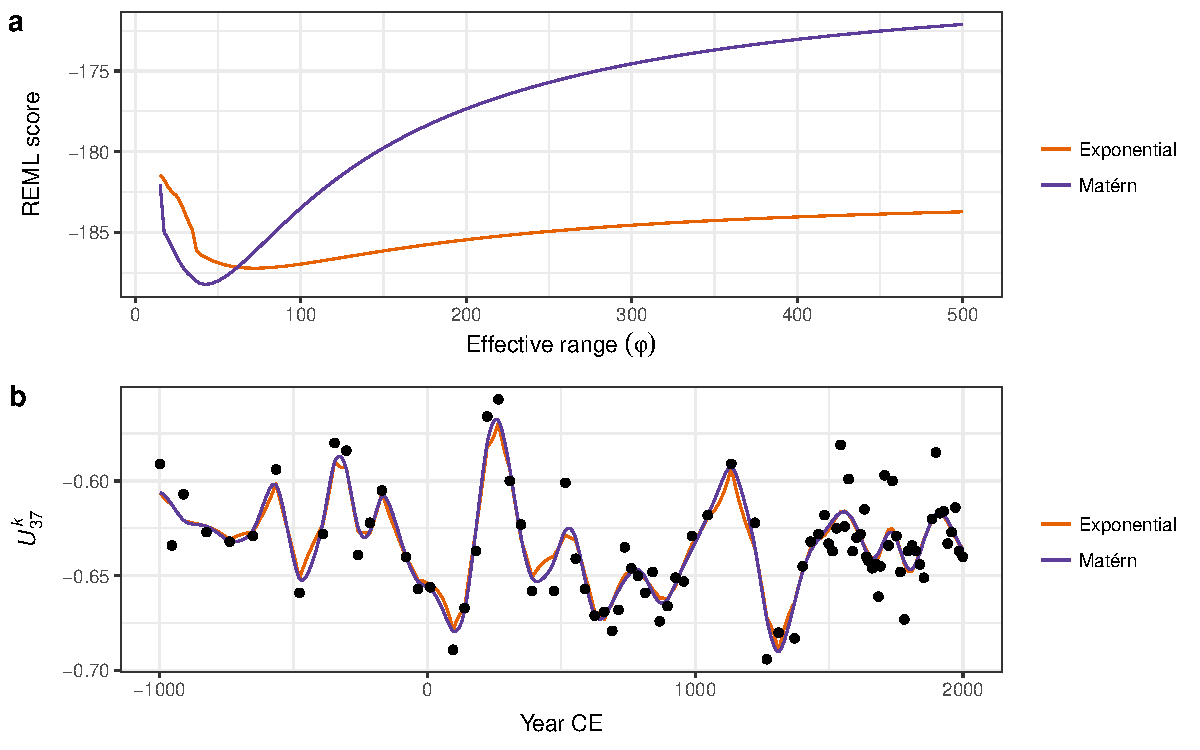
\includegraphics[width=0.8\linewidth]{supplementary-materials_files/figure-latex/gp-gam-detail-plot-1} \end{center}

Next we extract the minimum of the REML scores for the two correlation
functions and refit those models (we threw away all the models in the
\texttt{for\ ()} loop earlier to avoid storing lots of model objects).
Then we fit GAMs with Gaussian process smooths using the values of
\(\phi\) that produced the minimum REML scores, and predict using the
fitted models to visualize the trends.

\begin{Shaded}
\begin{Highlighting}[]
\NormalTok{effRange1 <-}\StringTok{ }\DecValTok{250}      \CommentTok{# sets effective range in years for Matérn correl}
\NormalTok{## minima from profile likelihood}
\NormalTok{effRange2 <-}\StringTok{ }\KeywordTok{with}\NormalTok{(}\KeywordTok{subset}\NormalTok{(reml.scr, cor ==}\StringTok{ "Matérn"}\NormalTok{), dseq[}\KeywordTok{which.min}\NormalTok{(reml)])}
\NormalTok{effRange3 <-}\StringTok{ }\KeywordTok{with}\NormalTok{(}\KeywordTok{subset}\NormalTok{(reml.scr, cor ==}\StringTok{ "Exponential"}\NormalTok{), dseq[}\KeywordTok{which.min}\NormalTok{(reml)])}

\NormalTok{## Matern}
\NormalTok{gp2 <-}\StringTok{ }\KeywordTok{gam}\NormalTok{(UK37 ~}\StringTok{ }\KeywordTok{s}\NormalTok{(Year, }\DataTypeTok{k =} \DecValTok{45}\NormalTok{, }\DataTypeTok{bs =} \StringTok{"gp"}\NormalTok{, }\DataTypeTok{m =} \KeywordTok{c}\NormalTok{(}\DecValTok{3}\NormalTok{, effRange2)),}
           \DataTypeTok{data =} \NormalTok{braya,}
           \DataTypeTok{method =} \StringTok{"REML"}\NormalTok{, }\DataTypeTok{weights =} \NormalTok{sampleInterval /}\StringTok{ }\KeywordTok{mean}\NormalTok{(sampleInterval))}
\NormalTok{## Power exponential}
\NormalTok{gp3 <-}\StringTok{ }\KeywordTok{gam}\NormalTok{(UK37 ~}\StringTok{ }\KeywordTok{s}\NormalTok{(Year, }\DataTypeTok{k =} \DecValTok{45}\NormalTok{, }\DataTypeTok{bs =} \StringTok{"gp"}\NormalTok{, }\DataTypeTok{m =} \KeywordTok{c}\NormalTok{(}\DecValTok{2}\NormalTok{, effRange3, }\DecValTok{1}\NormalTok{)),}
           \DataTypeTok{data =} \NormalTok{braya,}
           \DataTypeTok{method =} \StringTok{"REML"}\NormalTok{, }\DataTypeTok{weights =} \NormalTok{sampleInterval /}\StringTok{ }\KeywordTok{mean}\NormalTok{(sampleInterval))}

\NormalTok{newd <-}\StringTok{ }\KeywordTok{with}\NormalTok{(braya, }\KeywordTok{data.frame}\NormalTok{(}\DataTypeTok{Year =} \KeywordTok{seq}\NormalTok{(}\KeywordTok{min}\NormalTok{(Year), }\KeywordTok{max}\NormalTok{(Year),}
                               \DataTypeTok{length.out =} \DecValTok{1000}\NormalTok{)))}
\NormalTok{p.gp2 <-}\StringTok{ }\KeywordTok{transform}\NormalTok{(newd,}
                   \DataTypeTok{fitted =} \KeywordTok{predict}\NormalTok{(gp2, }\DataTypeTok{newdata =} \NormalTok{newd, }\DataTypeTok{type =} \StringTok{"response"}\NormalTok{),}
                   \DataTypeTok{effRange =} \KeywordTok{round}\NormalTok{(effRange2))}
\NormalTok{p.gp3 <-}\StringTok{ }\KeywordTok{transform}\NormalTok{(newd,}
                   \DataTypeTok{fitted =} \KeywordTok{predict}\NormalTok{(gp3, }\DataTypeTok{newdata =} \NormalTok{newd, }\DataTypeTok{type =} \StringTok{"response"}\NormalTok{),}
                   \DataTypeTok{effRange =} \KeywordTok{round}\NormalTok{(effRange3))}
\NormalTok{## pred <- rbind(p.gp1, p.gp2, p.gp3)}
\NormalTok{pred <-}\StringTok{ }\KeywordTok{rbind}\NormalTok{(p.gp2, p.gp3)}
\NormalTok{pred <-}\StringTok{ }\KeywordTok{transform}\NormalTok{(pred, }\DataTypeTok{effRange =} \KeywordTok{factor}\NormalTok{(effRange),}
                  \DataTypeTok{cor =} \KeywordTok{rep}\NormalTok{(}\KeywordTok{c}\NormalTok{(}\StringTok{"Matérn"}\NormalTok{, }\StringTok{"Exponential"}\NormalTok{), }\DataTypeTok{each =} \KeywordTok{nrow}\NormalTok{(newd)))}
\end{Highlighting}
\end{Shaded}

The estimated trends are plotted using

\begin{Shaded}
\begin{Highlighting}[]
\NormalTok{## plot at two values of h}
\NormalTok{gp.plt2 <-}\StringTok{ }\KeywordTok{ggplot}\NormalTok{(pred, }\KeywordTok{aes}\NormalTok{(}\DataTypeTok{x =} \NormalTok{Year, }\DataTypeTok{y =} \NormalTok{fitted, }\DataTypeTok{colour =} \NormalTok{cor)) +}
\StringTok{    }\KeywordTok{geom_line}\NormalTok{() +}\StringTok{ }\KeywordTok{theme}\NormalTok{(}\DataTypeTok{legend.position =} \StringTok{"right"}\NormalTok{) +}
\StringTok{    }\KeywordTok{geom_point}\NormalTok{(}\KeywordTok{aes}\NormalTok{(}\DataTypeTok{x =} \NormalTok{Year, }\DataTypeTok{y =} \NormalTok{UK37), }\DataTypeTok{data =} \NormalTok{braya, }\DataTypeTok{inherit.aes =} \OtherTok{FALSE}\NormalTok{) +}
\StringTok{    }\KeywordTok{scale_colour_manual}\NormalTok{(}\DataTypeTok{name =} \StringTok{""}\NormalTok{, }\DataTypeTok{values =} \KeywordTok{c}\NormalTok{(}\StringTok{"#e66101"}\NormalTok{,}\StringTok{"#5e3c99"}\NormalTok{)) +}
\StringTok{    }\KeywordTok{labs}\NormalTok{(}\DataTypeTok{y =} \NormalTok{braya_ylabel, }\DataTypeTok{x =} \StringTok{"Year CE"}\NormalTok{)}
\end{Highlighting}
\end{Shaded}

whilst Figure 12 in the manuscript was prepared using

\begin{Shaded}
\begin{Highlighting}[]
\KeywordTok{plot_grid}\NormalTok{(proflik.plt, gp.plt2, }\DataTypeTok{ncol =} \DecValTok{1}\NormalTok{, }\DataTypeTok{labels =} \KeywordTok{c}\NormalTok{(}\StringTok{"a"}\NormalTok{,}\StringTok{"b"}\NormalTok{),}
          \DataTypeTok{align =} \StringTok{"hv"}\NormalTok{, }\DataTypeTok{axis =} \StringTok{"lr"}\NormalTok{)}
\end{Highlighting}
\end{Shaded}

\begin{center}\includegraphics[width=0.8\linewidth]{supplementary-materials_files/figure-latex/figure-12-1} \end{center}

\section{Adaptive smooths}\label{adaptive-smooths}

The adaptive smooth was fitted to the Braya-Sø data by adding
\texttt{bs\ =\ "ad"} to the \texttt{s()} term in the model formula. The
other aspects of the fit are as previously used for the other models,
REML smoothness selection and observational weights:

\begin{Shaded}
\begin{Highlighting}[]
\NormalTok{## Adaptive spline, weights as sampleInterval}
\NormalTok{mod_ad <-}\StringTok{ }\KeywordTok{gam}\NormalTok{(UK37 ~}\StringTok{ }\KeywordTok{s}\NormalTok{(Year, }\DataTypeTok{k =} \DecValTok{45}\NormalTok{, }\DataTypeTok{bs =} \StringTok{"ad"}\NormalTok{), }\DataTypeTok{data =} \NormalTok{braya,}
              \DataTypeTok{method =} \StringTok{"REML"}\NormalTok{,}
              \DataTypeTok{weights =} \NormalTok{sampleInterval /}\StringTok{ }\KeywordTok{mean}\NormalTok{(sampleInterval))}
\end{Highlighting}
\end{Shaded}

\section{Compare various trends}\label{compare-various-trends}

For the model comparison, I refitted all the models for consistency; the
code to fit each of the

\begin{enumerate}
\def\labelenumi{\arabic{enumi}.}
\tightlist
\item
  Thin plate regression spline,
\item
  Gaussian process spline (Matérn correlation functions), and
\item
  Adaptive smoother
\end{enumerate}

is shown below.

\begin{Shaded}
\begin{Highlighting}[]
\NormalTok{## model it using gam()}
\NormalTok{effRange <-}\StringTok{ }\NormalTok{effRange2}

\NormalTok{## TPRS, weights as sampleInterval, k = needs to be higher}
\NormalTok{mod_tprs <-}\StringTok{ }\KeywordTok{gam}\NormalTok{(UK37 ~}\StringTok{ }\KeywordTok{s}\NormalTok{(Year, }\DataTypeTok{k =} \DecValTok{45}\NormalTok{, }\DataTypeTok{bs =} \StringTok{"tp"}\NormalTok{), }\DataTypeTok{data =} \NormalTok{braya,}
                \DataTypeTok{method =} \StringTok{"REML"}\NormalTok{,}
                \DataTypeTok{weights =} \NormalTok{sampleInterval /}\StringTok{ }\KeywordTok{mean}\NormalTok{(sampleInterval))}

\NormalTok{## Gaussian process, Matern, kappa = 1.5, weights as sampleInterval}
\NormalTok{mod_gp <-}\StringTok{ }\KeywordTok{gam}\NormalTok{(UK37 ~}\StringTok{ }\KeywordTok{s}\NormalTok{(Year, }\DataTypeTok{k =} \DecValTok{45}\NormalTok{, }\DataTypeTok{bs =} \StringTok{"gp"}\NormalTok{, }\DataTypeTok{m =} \KeywordTok{c}\NormalTok{(}\DecValTok{3}\NormalTok{, effRange)),}
              \DataTypeTok{data =} \NormalTok{braya,}
              \DataTypeTok{method =} \StringTok{"REML"}\NormalTok{,}
              \DataTypeTok{weights =} \NormalTok{sampleInterval /}\StringTok{ }\KeywordTok{mean}\NormalTok{(sampleInterval))}

\NormalTok{## Adaptive spline, weights as sampleInterval}
\NormalTok{mod_ad <-}\StringTok{ }\KeywordTok{gam}\NormalTok{(UK37 ~}\StringTok{ }\KeywordTok{s}\NormalTok{(Year, }\DataTypeTok{k =} \DecValTok{45}\NormalTok{, }\DataTypeTok{bs =} \StringTok{"ad"}\NormalTok{), }\DataTypeTok{data =} \NormalTok{braya,}
              \DataTypeTok{method =} \StringTok{"REML"}\NormalTok{,}
              \DataTypeTok{weights =} \NormalTok{sampleInterval /}\StringTok{ }\KeywordTok{mean}\NormalTok{(sampleInterval))}
\end{Highlighting}
\end{Shaded}

We write a small function to predict from each model over the range of
\texttt{Year} and return the data in tidy format for plotting. The plot
produce reproduces figure 13 in the manuscript.

\begin{Shaded}
\begin{Highlighting}[]
\NormalTok{## wrap this in a function that will return all the plots & derived objects}
\NormalTok{processGAM <-}\StringTok{ }\NormalTok{function(mod) \{}
    \NormalTok{## Predict from model}
    \NormalTok{N <-}\StringTok{ }\DecValTok{500}
    \NormalTok{newYear <-}\StringTok{ }\KeywordTok{with}\NormalTok{(braya,}
                    \KeywordTok{data.frame}\NormalTok{(}\DataTypeTok{Year =} \KeywordTok{seq}\NormalTok{(}\KeywordTok{min}\NormalTok{(Year), }\KeywordTok{max}\NormalTok{(Year),}
                                          \DataTypeTok{length.out =} \NormalTok{N)))}
    \NormalTok{newYear <-}\StringTok{ }\KeywordTok{cbind}\NormalTok{(newYear,}
                     \KeywordTok{data.frame}\NormalTok{(}\KeywordTok{predict}\NormalTok{(mod, newYear, }\DataTypeTok{se.fit =} \OtherTok{TRUE}\NormalTok{)))}
    
    \NormalTok{out <-}\StringTok{ }\KeywordTok{list}\NormalTok{(}\DataTypeTok{objects =} \NormalTok{newYear)}
    \NormalTok{out}
\NormalTok{\}}

\NormalTok{plts_gp   <-}\StringTok{ }\KeywordTok{processGAM}\NormalTok{(}\DataTypeTok{mod =} \NormalTok{mod_gp) }\CommentTok{# Gaussian process smooth with weights}
\NormalTok{plts_ad   <-}\StringTok{ }\KeywordTok{processGAM}\NormalTok{(}\DataTypeTok{mod =} \NormalTok{mod_ad) }\CommentTok{# Adaptive smooth with weights}
\NormalTok{plts_tprs <-}\StringTok{ }\KeywordTok{processGAM}\NormalTok{(}\DataTypeTok{mod =} \NormalTok{mod_tprs) }\CommentTok{# TPRS with weights}

\NormalTok{pltData <-}\StringTok{ }\KeywordTok{do.call}\NormalTok{(}\StringTok{"rbind"}\NormalTok{, }\KeywordTok{lapply}\NormalTok{(}\KeywordTok{list}\NormalTok{(plts_gp, plts_ad, plts_tprs),}
                                   \StringTok{`}\DataTypeTok{[[}\StringTok{`}\NormalTok{, }\StringTok{"objects"}\NormalTok{))}
\NormalTok{pltData <-}\StringTok{ }\KeywordTok{transform}\NormalTok{(pltData, }\DataTypeTok{Model =} \KeywordTok{rep}\NormalTok{(}\KeywordTok{c}\NormalTok{(}\StringTok{"GP"}\NormalTok{, }\StringTok{"Adaptive"}\NormalTok{, }\StringTok{"TPRS"}\NormalTok{),}
                              \DataTypeTok{each =} \KeywordTok{nrow}\NormalTok{(plts_gp$objects)))}

\NormalTok{allFits <-}\StringTok{ }\KeywordTok{ggplot}\NormalTok{(pltData, }\KeywordTok{aes}\NormalTok{(}\DataTypeTok{x =} \NormalTok{Year, }\DataTypeTok{y =} \NormalTok{fit)) +}
\StringTok{    }\KeywordTok{geom_point}\NormalTok{(}\KeywordTok{aes}\NormalTok{(}\DataTypeTok{x =} \NormalTok{Year, }\DataTypeTok{y =} \NormalTok{UK37), }\DataTypeTok{data =} \NormalTok{braya) +}
\StringTok{    }\KeywordTok{geom_line}\NormalTok{(}\KeywordTok{aes}\NormalTok{(}\DataTypeTok{colour =} \NormalTok{Model)) +}\StringTok{ }\KeywordTok{labs}\NormalTok{(}\DataTypeTok{y =} \NormalTok{braya_ylabel, }\DataTypeTok{x =} \StringTok{"Year"}\NormalTok{) +}
\StringTok{    }\KeywordTok{theme}\NormalTok{(}\DataTypeTok{legend.position =} \StringTok{"right"}\NormalTok{) +}
\StringTok{    }\KeywordTok{scale_colour_manual}\NormalTok{(}\DataTypeTok{name =} \StringTok{""}\NormalTok{,}
                        \DataTypeTok{values =} \KeywordTok{c}\NormalTok{(}\StringTok{"#e66101"}\NormalTok{, }\StringTok{"#fdb863"}\NormalTok{, }\StringTok{"#5e3c99"}\NormalTok{))}
\NormalTok{allFits}
\end{Highlighting}
\end{Shaded}

\begin{center}\includegraphics[width=0.8\linewidth]{supplementary-materials_files/figure-latex/process-models-1} \end{center}

\section{Accounting for age-model
uncertainty}\label{accounting-for-age-model-uncertainty}

The manuscript proposed to simulate from the posterior distribution of
the fitted age model as a way to account for age-model uncertainty. The
first step in the process is to fit the age model from which to simulate
new age models. This was done using the \emph{scam} package for a
\emph{shape-constrained GAM}, with the age-model spline constrained to
be monotonic decreasing (\texttt{bs\ =\ "mpd"}).

To make this section self-contained, I refitted the Small Water GAM plus
CAR(1) model

\begin{Shaded}
\begin{Highlighting}[]
\NormalTok{knots <-}\StringTok{ }\KeywordTok{with}\NormalTok{(small, }\KeywordTok{list}\NormalTok{(}\DataTypeTok{Year =} \KeywordTok{seq}\NormalTok{(}\KeywordTok{min}\NormalTok{(Year), }\KeywordTok{max}\NormalTok{(Year), }\DataTypeTok{length =} \DecValTok{14}\NormalTok{)))}
\NormalTok{mod <-}\StringTok{ }\KeywordTok{gamm}\NormalTok{(d15N ~}\StringTok{ }\KeywordTok{s}\NormalTok{(Year, }\DataTypeTok{k =} \DecValTok{15}\NormalTok{), }\DataTypeTok{data =} \NormalTok{small, }\DataTypeTok{method =} \StringTok{"REML"}\NormalTok{,}
            \DataTypeTok{correlation =} \KeywordTok{corCAR1}\NormalTok{(}\DataTypeTok{form =} \NormalTok{~}\StringTok{ }\NormalTok{Year),}
            \DataTypeTok{knots =} \NormalTok{knots)}
\end{Highlighting}
\end{Shaded}

and then we load the \textsuperscript{210}Pb dating results for the
dated core sections.

\begin{Shaded}
\begin{Highlighting}[]
\NormalTok{swAge <-}\StringTok{ }\KeywordTok{read.csv}\NormalTok{(}\StringTok{"./data/small-water/small1-dating.csv"}\NormalTok{)}
\end{Highlighting}
\end{Shaded}

before fitting the shape-constrained GAM. Currently, \emph{scam} can
only fit models using GCV smoothness selection. I used the
\texttt{gamma} argument here to add a larger penalty for more-complex
models. Each effective degree of freedom used by the spline is counted
as 1.4 degrees of freedom in the GCV score.

\begin{Shaded}
\begin{Highlighting}[]
\NormalTok{## monotonic spline age-depth model}
\NormalTok{swAge$Error[}\DecValTok{1}\NormalTok{] <-}\StringTok{ }\FloatTok{1.1}
\NormalTok{swAgeMod <-}\StringTok{ }\KeywordTok{scam}\NormalTok{(Date ~}\StringTok{ }\KeywordTok{s}\NormalTok{(Depth, }\DataTypeTok{k =} \DecValTok{5}\NormalTok{, }\DataTypeTok{bs =} \StringTok{"mpd"}\NormalTok{), }\DataTypeTok{data =} \NormalTok{swAge,}
                 \DataTypeTok{weights =} \DecValTok{1} \NormalTok{/}\StringTok{ }\NormalTok{swAge$Error, }\DataTypeTok{gamma =} \FloatTok{1.4}\NormalTok{)}
\end{Highlighting}
\end{Shaded}

Note that I added a small amount of error to the surface sample age as
the model cannot be fitted if an observation has \texttt{0} weight.

Next, predict from the estimated age model, and draw 25 samples from the
posterior distribution using \texttt{simulate()}. The results are tidied
into a format suitable for further processing and plotting. Note that
the posterior samples here are only used for plotting.

\begin{Shaded}
\begin{Highlighting}[]
\NormalTok{## predict from the age model for a smooth set of points in `Depth`}
\NormalTok{newAge <-}\StringTok{ }\KeywordTok{with}\NormalTok{(swAge, }\KeywordTok{data.frame}\NormalTok{(}\DataTypeTok{Depth =} \KeywordTok{seq}\NormalTok{(}\KeywordTok{min}\NormalTok{(Depth), }\KeywordTok{max}\NormalTok{(Depth),}
                                             \DataTypeTok{length.out =} \DecValTok{200}\NormalTok{)))}
\NormalTok{newAge <-}\StringTok{ }\KeywordTok{transform}\NormalTok{(newAge,}
                    \DataTypeTok{fitted =} \KeywordTok{predict}\NormalTok{(swAgeMod, }\DataTypeTok{newdata =} \NormalTok{newAge, }
                                     \DataTypeTok{type =} \StringTok{"response"}\NormalTok{))}
\NormalTok{newSims <-}\StringTok{ }\KeywordTok{as.data.frame}\NormalTok{(}\KeywordTok{simulate}\NormalTok{(swAgeMod, }\DataTypeTok{nsim =} \DecValTok{25}\NormalTok{, }\DataTypeTok{newdata =} \NormalTok{newAge))}
\NormalTok{newSims <-}\StringTok{ }\KeywordTok{cbind}\NormalTok{(}\DataTypeTok{Depth =} \NormalTok{newAge$Depth, newSims)}
\NormalTok{newSims <-}\StringTok{ }\KeywordTok{gather}\NormalTok{(newSims, Simulation, Age, -Depth)}
\end{Highlighting}
\end{Shaded}

In the next code chunk, I draw 100 samples from the posterior
distribution of the age model, but notice that I pass in the
\texttt{small} data to \texttt{newdata} in the call to
\texttt{simulate()} as the locations I want new age estimates for are
the depths for which we have δ\textsuperscript{15}N values. A small
function (\texttt{fitSWModels}) is written to prepare each simulation
for fitting and then actually fit the GAM plus CAR(1) model using the
updated age information.

\begin{Shaded}
\begin{Highlighting}[]
\NormalTok{## simulate from age model; each column is a simulation}
\NormalTok{ageSims <-}\StringTok{ }\KeywordTok{simulate}\NormalTok{(swAgeMod, }\DataTypeTok{nsim =} \DecValTok{100}\NormalTok{, }\DataTypeTok{newdata =} \NormalTok{small, }\DataTypeTok{seed =} \DecValTok{42}\NormalTok{)}
\NormalTok{ageSims <-}\StringTok{ }\KeywordTok{as.data.frame}\NormalTok{(ageSims)}

\NormalTok{fitSWModels <-}\StringTok{ }\NormalTok{function(x, y, knots) \{}
    \NormalTok{dat <-}\StringTok{ }\KeywordTok{data.frame}\NormalTok{(}\DataTypeTok{d15N =} \NormalTok{y, }\DataTypeTok{Year =} \NormalTok{x)}
    \NormalTok{m <-}\StringTok{ }\KeywordTok{gamm}\NormalTok{(d15N ~}\StringTok{ }\KeywordTok{s}\NormalTok{(Year, }\DataTypeTok{k =} \DecValTok{15}\NormalTok{), }\DataTypeTok{data =} \NormalTok{dat, }\DataTypeTok{method =} \StringTok{"REML"}\NormalTok{,}
              \DataTypeTok{correlation =} \KeywordTok{corCAR1}\NormalTok{(}\DataTypeTok{form =} \NormalTok{~}\StringTok{ }\NormalTok{Year), }\DataTypeTok{knots =} \NormalTok{knots)}
\NormalTok{\}}

\NormalTok{## generate new trends using draws from age-model posterior}
\NormalTok{simTrendMods <-}\StringTok{ }\KeywordTok{lapply}\NormalTok{(ageSims, fitSWModels, }\DataTypeTok{y =} \NormalTok{small$d15N, }\DataTypeTok{knots =} \NormalTok{knots)}


\NormalTok{## function wrapper to predict new trends at locations over the}
\NormalTok{## range of `Year`}
\NormalTok{predSWModels <-}\StringTok{ }\NormalTok{function(mod, newdata) \{}
    \KeywordTok{predict}\NormalTok{(mod$gam, }\DataTypeTok{newdata =} \NormalTok{newdata, }\DataTypeTok{type =} \StringTok{"response"}\NormalTok{)}
\NormalTok{\}}

\NormalTok{## predict from fitted model to produce a smooth trend for each posterior}
\NormalTok{## sample}
\NormalTok{simTrends <-}\StringTok{ }\KeywordTok{lapply}\NormalTok{(simTrendMods, predSWModels, }\DataTypeTok{newdata =} \NormalTok{newYear)}

\NormalTok{## arrange in a tidy format form plottings}
\NormalTok{simTrends <-}\StringTok{ }\KeywordTok{data.frame}\NormalTok{(}\DataTypeTok{Year  =} \KeywordTok{with}\NormalTok{(newYear, }\KeywordTok{rep}\NormalTok{(Year, }\KeywordTok{length}\NormalTok{(simTrends))),}
                        \DataTypeTok{Trend =} \KeywordTok{unlist}\NormalTok{(simTrends),}
                        \DataTypeTok{Group =} \KeywordTok{rep}\NormalTok{(}\KeywordTok{seq_along}\NormalTok{(simTrends),}
                                    \DataTypeTok{times =} \KeywordTok{lengths}\NormalTok{(simTrends)))}
\end{Highlighting}
\end{Shaded}

The next chunk does the final step in the process. For each of the
models we just fitted to include age model uncertainty, we simulate 50
draws from the model posterior distribution. We start with a wrapper
function around the \texttt{simulate()} code we want to run on each
model, then do the actual posterior draws for each model using
\texttt{lapply()}. The final step just arranges data for plotting.

\begin{Shaded}
\begin{Highlighting}[]
\NormalTok{## wrapper to simulate from a fitted GAM with the arguments/settings}
\NormalTok{## I want}
\NormalTok{simulateSWModels <-}\StringTok{ }\NormalTok{function(mod, newdata, nsim, }\DataTypeTok{seed =} \DecValTok{42}\NormalTok{) \{}
    \NormalTok{sims <-}\StringTok{ }\KeywordTok{simulate}\NormalTok{(mod, }\DataTypeTok{nsim =} \NormalTok{nsim, }\DataTypeTok{newdata =} \NormalTok{newdata, }\DataTypeTok{seed =} \NormalTok{seed)}
    \KeywordTok{as.vector}\NormalTok{(sims)}
\NormalTok{\}}

\NormalTok{## now do the posterior simulation}
\NormalTok{NSIM <-}\StringTok{ }\DecValTok{50}     \CommentTok{# number of posterior samples *per* model}
\NormalTok{simSimulate <-}\StringTok{ }\KeywordTok{lapply}\NormalTok{(simTrendMods, simulateSWModels, }\DataTypeTok{newdata =} \NormalTok{newYear,}
                      \DataTypeTok{nsim =} \NormalTok{NSIM, }\DataTypeTok{seed =} \DecValTok{42}\NormalTok{)}

\NormalTok{## arrange in a tidy format}
\NormalTok{simSimulate <-}
\StringTok{  }\KeywordTok{data.frame}\NormalTok{(}\DataTypeTok{Year  =} \KeywordTok{with}\NormalTok{(newYear,}
                          \KeywordTok{rep}\NormalTok{(Year, }\DataTypeTok{times =} \NormalTok{NSIM *}\StringTok{ }\KeywordTok{length}\NormalTok{(simSimulate))),}
             \DataTypeTok{Trend =} \KeywordTok{unlist}\NormalTok{(simSimulate),}
             \DataTypeTok{Group =} \KeywordTok{rep}\NormalTok{(}\KeywordTok{seq_len}\NormalTok{(NSIM *}\StringTok{ }\KeywordTok{length}\NormalTok{(simSimulate)),}
                         \DataTypeTok{each =} \KeywordTok{nrow}\NormalTok{(newYear)))}
\end{Highlighting}
\end{Shaded}

Each of the steps is visualized using the plot code shown below.

\begin{Shaded}
\begin{Highlighting}[]
\NormalTok{plt1 <-}\StringTok{ }\KeywordTok{ggplot}\NormalTok{(swAge, }\KeywordTok{aes}\NormalTok{(}\DataTypeTok{y =} \NormalTok{Date, }\DataTypeTok{x =} \NormalTok{Depth)) +}
\StringTok{    }\KeywordTok{geom_line}\NormalTok{(}\DataTypeTok{data =} \NormalTok{newSims,}
              \DataTypeTok{mapping =} \KeywordTok{aes}\NormalTok{(}\DataTypeTok{y =} \NormalTok{Age, }\DataTypeTok{x =} \NormalTok{Depth, }\DataTypeTok{group =} \NormalTok{Simulation),}
              \DataTypeTok{alpha =} \DecValTok{1}\NormalTok{, }\DataTypeTok{colour =} \StringTok{"grey80"}\NormalTok{) +}
\StringTok{    }\KeywordTok{geom_line}\NormalTok{(}\DataTypeTok{data =} \NormalTok{newAge, }\DataTypeTok{mapping =} \KeywordTok{aes}\NormalTok{(}\DataTypeTok{y =} \NormalTok{fitted, }\DataTypeTok{x =} \NormalTok{Depth)) +}
\StringTok{    }\KeywordTok{geom_point}\NormalTok{(}\DataTypeTok{size =} \FloatTok{1.5}\NormalTok{, }\DataTypeTok{colour =} \StringTok{"red"}\NormalTok{) +}
\StringTok{    }\KeywordTok{geom_errorbar}\NormalTok{(}\KeywordTok{aes}\NormalTok{(}\DataTypeTok{ymin =} \NormalTok{Date -}\StringTok{ }\NormalTok{Error, }\DataTypeTok{ymax =} \NormalTok{Date +}\StringTok{ }\NormalTok{Error, }\DataTypeTok{width =} \DecValTok{0}\NormalTok{),}
                  \DataTypeTok{colour =} \StringTok{"red"}\NormalTok{) +}
\StringTok{    }\KeywordTok{labs}\NormalTok{(}\DataTypeTok{y =} \StringTok{"Year CE"}\NormalTok{, }\DataTypeTok{x =} \StringTok{"Depth (cm)"}\NormalTok{)}

\NormalTok{plt2 <-}\StringTok{ }\KeywordTok{ggplot}\NormalTok{(simTrends, }\KeywordTok{aes}\NormalTok{(}\DataTypeTok{x =} \NormalTok{Year, }\DataTypeTok{y =} \NormalTok{Trend, }\DataTypeTok{group =} \NormalTok{Group)) +}
\StringTok{    }\KeywordTok{geom_line}\NormalTok{(}\DataTypeTok{alpha =} \FloatTok{0.1}\NormalTok{, }\DataTypeTok{colour =} \StringTok{"grey80"}\NormalTok{) +}
\StringTok{    }\KeywordTok{geom_line}\NormalTok{(}\DataTypeTok{data =} \NormalTok{newYear,}
              \DataTypeTok{mapping =} \KeywordTok{aes}\NormalTok{(}\DataTypeTok{x =} \NormalTok{Year, }\DataTypeTok{y =} \NormalTok{fit), }\DataTypeTok{inherit.aes =} \OtherTok{FALSE}\NormalTok{) +}
\StringTok{    }\KeywordTok{geom_point}\NormalTok{(}\DataTypeTok{data =} \NormalTok{small,}
               \DataTypeTok{mapping =} \KeywordTok{aes}\NormalTok{(}\DataTypeTok{x =} \NormalTok{Year, }\DataTypeTok{y =} \NormalTok{d15N),}
               \DataTypeTok{inherit.aes =} \OtherTok{FALSE}\NormalTok{, }\DataTypeTok{size =} \FloatTok{0.7}\NormalTok{) +}
\StringTok{    }\KeywordTok{labs}\NormalTok{(}\DataTypeTok{x =} \StringTok{"Year"}\NormalTok{, }\DataTypeTok{y =} \NormalTok{d15n_label)}

\NormalTok{plt3 <-}\StringTok{ }\KeywordTok{ggplot}\NormalTok{(simSimulate, }\KeywordTok{aes}\NormalTok{(}\DataTypeTok{x =} \NormalTok{Year, }\DataTypeTok{y =} \NormalTok{Trend, }\DataTypeTok{group =} \NormalTok{Group)) +}
\StringTok{    }\KeywordTok{geom_line}\NormalTok{(}\DataTypeTok{alpha =} \FloatTok{0.2}\NormalTok{, }\DataTypeTok{colour =} \StringTok{"grey80"}\NormalTok{) +}
\StringTok{    }\KeywordTok{geom_point}\NormalTok{(}\DataTypeTok{data =} \NormalTok{small,}
               \DataTypeTok{mapping =} \KeywordTok{aes}\NormalTok{(}\DataTypeTok{x =} \NormalTok{Year, }\DataTypeTok{y =} \NormalTok{d15N),}
               \DataTypeTok{inherit.aes =} \OtherTok{FALSE}\NormalTok{,}
               \DataTypeTok{size =} \FloatTok{0.7}\NormalTok{) +}
\StringTok{    }\KeywordTok{geom_line}\NormalTok{(}\DataTypeTok{data =} \NormalTok{newYear,}
              \DataTypeTok{mapping =} \KeywordTok{aes}\NormalTok{(}\DataTypeTok{x =} \NormalTok{Year, }\DataTypeTok{y =} \NormalTok{fit),}
              \DataTypeTok{inherit.aes =} \OtherTok{FALSE}\NormalTok{) +}
\StringTok{    }\KeywordTok{labs}\NormalTok{(}\DataTypeTok{x =} \StringTok{"Year"}\NormalTok{, }\DataTypeTok{y =} \NormalTok{d15n_label)}

\KeywordTok{plot_grid}\NormalTok{(plt1, plt2, plt3, }\DataTypeTok{ncol =} \DecValTok{1}\NormalTok{, }\DataTypeTok{labels =} \StringTok{"auto"}\NormalTok{, }\DataTypeTok{align =} \StringTok{"hv"}\NormalTok{,}
          \DataTypeTok{axis =} \StringTok{"lrtb"}\NormalTok{, }\DataTypeTok{rel_widths =} \KeywordTok{c}\NormalTok{(}\FloatTok{0.5}\NormalTok{, }\DecValTok{1}\NormalTok{, }\DecValTok{1}\NormalTok{))}
\end{Highlighting}
\end{Shaded}

\begin{center}\includegraphics[width=0.8\linewidth]{supplementary-materials_files/figure-latex/small-scam-fit-plots-1} \end{center}

This reproduces figure 14 from the manuscript.

\section{Session information}\label{session-information}

\begin{Shaded}
\begin{Highlighting}[]
\NormalTok{devtools::}\KeywordTok{session_info}\NormalTok{()}
\end{Highlighting}
\end{Shaded}

\begin{verbatim}
#> Session info -------------------------------------------------------------
\end{verbatim}

\begin{verbatim}
#>  setting  value                                      
#>  version  R version 3.4.4 Patched (2018-03-17 r74422)
#>  system   x86_64, linux-gnu                          
#>  ui       X11                                        
#>  language (EN)                                       
#>  collate  en_CA.UTF-8                                
#>  tz       America/Regina                             
#>  date     2018-05-14
\end{verbatim}

\begin{verbatim}
#> Packages -----------------------------------------------------------------
\end{verbatim}

\begin{verbatim}
#>  package    * version date       source                                  
#>  backports    1.1.2   2017-12-13 CRAN (R 3.4.3)                          
#>  base       * 3.4.4   2018-03-18 local                                   
#>  codetools    0.2-15  2016-10-05 CRAN (R 3.4.4)                          
#>  colorspace   1.3-2   2016-12-14 CRAN (R 3.4.1)                          
#>  compiler     3.4.4   2018-03-18 local                                   
#>  cowplot    * 0.9.2   2017-12-17 CRAN (R 3.4.3)                          
#>  datasets   * 3.4.4   2018-03-18 local                                   
#>  devtools     1.13.5  2018-02-18 CRAN (R 3.4.4)                          
#>  digest       0.6.15  2018-01-28 CRAN (R 3.4.4)                          
#>  evaluate     0.10.1  2017-06-24 CRAN (R 3.4.1)                          
#>  ggplot2    * 2.2.1   2016-12-30 CRAN (R 3.4.1)                          
#>  glue         1.2.0   2017-10-29 CRAN (R 3.4.2)                          
#>  graphics   * 3.4.4   2018-03-18 local                                   
#>  grDevices  * 3.4.4   2018-03-18 local                                   
#>  grid         3.4.4   2018-03-18 local                                   
#>  gtable       0.2.0   2016-02-26 CRAN (R 3.4.1)                          
#>  htmltools    0.3.6   2017-04-28 CRAN (R 3.4.1)                          
#>  knitr        1.20    2018-02-20 CRAN (R 3.4.4)                          
#>  labeling     0.3     2014-08-23 CRAN (R 3.4.1)                          
#>  lattice      0.20-35 2017-03-25 CRAN (R 3.4.4)                          
#>  lazyeval     0.2.1   2017-10-29 CRAN (R 3.4.2)                          
#>  magrittr     1.5     2014-11-22 CRAN (R 3.4.1)                          
#>  MASS         7.3-49  2018-02-23 CRAN (R 3.4.4)                          
#>  Matrix       1.2-14  2018-04-09 CRAN (R 3.4.4)                          
#>  memoise      1.1.0   2017-04-21 CRAN (R 3.4.1)                          
#>  methods      3.4.4   2018-03-18 local                                   
#>  mgcv       * 1.8-23  2018-01-21 CRAN (R 3.4.4)                          
#>  munsell      0.4.3   2016-02-13 CRAN (R 3.4.1)                          
#>  nlme       * 3.1-137 2018-04-07 CRAN (R 3.4.4)                          
#>  pillar       1.2.1   2018-02-27 CRAN (R 3.4.4)                          
#>  plyr         1.8.4   2016-06-08 CRAN (R 3.4.1)                          
#>  purrr        0.2.4   2017-10-18 CRAN (R 3.4.2)                          
#>  Rcpp         0.12.16 2018-03-13 CRAN (R 3.4.4)                          
#>  rlang        0.2.0   2018-02-20 CRAN (R 3.4.4)                          
#>  rmarkdown  * 1.9     2018-03-01 CRAN (R 3.4.4)                          
#>  rprojroot    1.3-2   2018-01-03 CRAN (R 3.4.3)                          
#>  scales       0.5.0   2017-08-24 CRAN (R 3.4.1)                          
#>  scam       * 1.2-2   2017-09-24 CRAN (R 3.4.3)                          
#>  schoenberg * 0.0-6   2018-04-12 Github (gavinsimpson/schoenberg@f9b8a84)
#>  splines      3.4.4   2018-03-18 local                                   
#>  stats      * 3.4.4   2018-03-18 local                                   
#>  stringi      1.1.7   2018-03-12 CRAN (R 3.4.4)                          
#>  stringr      1.3.0   2018-02-19 CRAN (R 3.4.4)                          
#>  tibble       1.4.2   2018-01-22 CRAN (R 3.4.3)                          
#>  tidyr      * 0.8.0   2018-01-29 CRAN (R 3.4.4)                          
#>  tools        3.4.4   2018-03-18 local                                   
#>  utils      * 3.4.4   2018-03-18 local                                   
#>  withr        2.1.2   2018-03-15 CRAN (R 3.4.4)                          
#>  yaml         2.1.18  2018-03-08 CRAN (R 3.4.4)
\end{verbatim}


\end{document}
